\documentclass{article}

\usepackage{arxiv}

\usepackage[utf8]{inputenc} % allow utf-8 input
\usepackage[T1]{fontenc}    % use 8-bit T1 fonts
\usepackage{lmodern}        % https://github.com/rstudio/rticles/issues/343
\usepackage{hyperref}       % hyperlinks
\usepackage{url}            % simple URL typesetting
\usepackage{booktabs}       % professional-quality tables
\usepackage{amsfonts}       % blackboard math symbols
\usepackage{nicefrac}       % compact symbols for 1/2, etc.
\usepackage{microtype}      % microtypography
\usepackage{graphicx}

\title{Predictive Approaches to Treatment Effect Heterogeneity}

\author{
    Tom Delany
    \thanks{\url{https://github.com/tomdelany04/PATH-Master}}
   \\
    Department of Mathematical and Statistical Sciences \\
    University of Galway \\
  Galway, Ireland \\
  \texttt{\href{mailto:d.tom2@universityofgalway.ie}{\nolinkurl{d.tom2@universityofgalway.ie}}} \\
   \And
    Misgana Ojamo
   \\
    Department of Mathematical and Statistical Sciences \\
    University of Galway \\
  Galway, Ireland \\
  \texttt{\href{mailto:M.Ojamo1@universityofgalway.ie}{\nolinkurl{M.Ojamo1@universityofgalway.ie}}} \\
  }

% Pandoc syntax highlighting
\usepackage{color}
\usepackage{fancyvrb}
\newcommand{\VerbBar}{|}
\newcommand{\VERB}{\Verb[commandchars=\\\{\}]}
\DefineVerbatimEnvironment{Highlighting}{Verbatim}{commandchars=\\\{\}}
% Add ',fontsize=\small' for more characters per line
\usepackage{framed}
\definecolor{shadecolor}{RGB}{248,248,248}
\newenvironment{Shaded}{\begin{snugshade}}{\end{snugshade}}
\newcommand{\AlertTok}[1]{\textcolor[rgb]{0.94,0.16,0.16}{#1}}
\newcommand{\AnnotationTok}[1]{\textcolor[rgb]{0.56,0.35,0.01}{\textbf{\textit{#1}}}}
\newcommand{\AttributeTok}[1]{\textcolor[rgb]{0.13,0.29,0.53}{#1}}
\newcommand{\BaseNTok}[1]{\textcolor[rgb]{0.00,0.00,0.81}{#1}}
\newcommand{\BuiltInTok}[1]{#1}
\newcommand{\CharTok}[1]{\textcolor[rgb]{0.31,0.60,0.02}{#1}}
\newcommand{\CommentTok}[1]{\textcolor[rgb]{0.56,0.35,0.01}{\textit{#1}}}
\newcommand{\CommentVarTok}[1]{\textcolor[rgb]{0.56,0.35,0.01}{\textbf{\textit{#1}}}}
\newcommand{\ConstantTok}[1]{\textcolor[rgb]{0.56,0.35,0.01}{#1}}
\newcommand{\ControlFlowTok}[1]{\textcolor[rgb]{0.13,0.29,0.53}{\textbf{#1}}}
\newcommand{\DataTypeTok}[1]{\textcolor[rgb]{0.13,0.29,0.53}{#1}}
\newcommand{\DecValTok}[1]{\textcolor[rgb]{0.00,0.00,0.81}{#1}}
\newcommand{\DocumentationTok}[1]{\textcolor[rgb]{0.56,0.35,0.01}{\textbf{\textit{#1}}}}
\newcommand{\ErrorTok}[1]{\textcolor[rgb]{0.64,0.00,0.00}{\textbf{#1}}}
\newcommand{\ExtensionTok}[1]{#1}
\newcommand{\FloatTok}[1]{\textcolor[rgb]{0.00,0.00,0.81}{#1}}
\newcommand{\FunctionTok}[1]{\textcolor[rgb]{0.13,0.29,0.53}{\textbf{#1}}}
\newcommand{\ImportTok}[1]{#1}
\newcommand{\InformationTok}[1]{\textcolor[rgb]{0.56,0.35,0.01}{\textbf{\textit{#1}}}}
\newcommand{\KeywordTok}[1]{\textcolor[rgb]{0.13,0.29,0.53}{\textbf{#1}}}
\newcommand{\NormalTok}[1]{#1}
\newcommand{\OperatorTok}[1]{\textcolor[rgb]{0.81,0.36,0.00}{\textbf{#1}}}
\newcommand{\OtherTok}[1]{\textcolor[rgb]{0.56,0.35,0.01}{#1}}
\newcommand{\PreprocessorTok}[1]{\textcolor[rgb]{0.56,0.35,0.01}{\textit{#1}}}
\newcommand{\RegionMarkerTok}[1]{#1}
\newcommand{\SpecialCharTok}[1]{\textcolor[rgb]{0.81,0.36,0.00}{\textbf{#1}}}
\newcommand{\SpecialStringTok}[1]{\textcolor[rgb]{0.31,0.60,0.02}{#1}}
\newcommand{\StringTok}[1]{\textcolor[rgb]{0.31,0.60,0.02}{#1}}
\newcommand{\VariableTok}[1]{\textcolor[rgb]{0.00,0.00,0.00}{#1}}
\newcommand{\VerbatimStringTok}[1]{\textcolor[rgb]{0.31,0.60,0.02}{#1}}
\newcommand{\WarningTok}[1]{\textcolor[rgb]{0.56,0.35,0.01}{\textbf{\textit{#1}}}}

% tightlist command for lists without linebreak
\providecommand{\tightlist}{%
  \setlength{\itemsep}{0pt}\setlength{\parskip}{0pt}}


% Pandoc citation processing
%From Pandoc 3.1.8
% definitions for citeproc citations
\NewDocumentCommand\citeproctext{}{}
\NewDocumentCommand\citeproc{mm}{%
  \begingroup\def\citeproctext{#2}\cite{#1}\endgroup}
\makeatletter
 % allow citations to break across lines
 \let\@cite@ofmt\@firstofone
 % avoid brackets around text for \cite:
 \def\@biblabel#1{}
 \def\@cite#1#2{{#1\if@tempswa , #2\fi}}
\makeatother
\newlength{\cslhangindent}
\setlength{\cslhangindent}{1.5em}
\newlength{\csllabelwidth}
\setlength{\csllabelwidth}{3em}
\newenvironment{CSLReferences}[2] % #1 hanging-indent, #2 entry-spacing
 {\begin{list}{}{%
  \setlength{\itemindent}{0pt}
  \setlength{\leftmargin}{0pt}
  \setlength{\parsep}{0pt}
  % turn on hanging indent if param 1 is 1
  \ifodd #1
   \setlength{\leftmargin}{\cslhangindent}
   \setlength{\itemindent}{-1\cslhangindent}
  \fi
  % set entry spacing
  \setlength{\itemsep}{#2\baselineskip}}}
 {\end{list}}
\usepackage{calc}
\newcommand{\CSLBlock}[1]{#1\hfill\break}
\newcommand{\CSLLeftMargin}[1]{\parbox[t]{\csllabelwidth}{#1}}
\newcommand{\CSLRightInline}[1]{\parbox[t]{\linewidth - \csllabelwidth}{#1}\break}
\newcommand{\CSLIndent}[1]{\hspace{\cslhangindent}#1}

\providecommand{\pandocbounded}[1]{#1}
\usepackage[HTML]{xcolor}
\usepackage{amsmath}
\usepackage{float}
\usepackage{placeins}
\usepackage{booktabs}
\usepackage{caption}
\usepackage{longtable}
\usepackage{colortbl}
\usepackage{array}
\usepackage{anyfontsize}
\usepackage{multirow}
\begin{document}
\maketitle


\begin{abstract}
Treatment effects observed in randomized controlled trials often vary
according to patients' baseline risk and other clinically prognostic
characteristics. Despite this heterogeneity of treatment effect, trial
findings are typically reported as a single average treatment effect,
while conventional subgroup analyses are limited by multiplicity, low
statistical power, and poor reproducibility. The Predictive Approaches
to Treatment Effect Heterogeneity (PATH) framework was developed to
address these limitations through multivariable risk modelling and
predictive analyses of treatment benefit across differing levels of
baseline risk.

The PATH framework was implemented across four large cardiovascular
trials (GUSTO-I, IST-I, DIG, and VITAL) with differing clinical
endpoints and outcome structures. Predictive risk models were used to
evaluate treatment effects across baseline-risk strata, while a Monte
Carlo simulation study was conducted to investigate the Type I error
performance of risk-based interaction testing.

Evidence of treatment-effect heterogeneity on the absolute scale was
observed in the GUSTO-I trial and, to a lesser extent, the IST-I trial,
where higher-risk patients derived greater absolute treatment benefit.
In contrast, the DIG and VITAL trials showed little evidence of
clinically meaningful heterogeneity, consistent with their limited
overall treatment effects. Simulation results demonstrated elevated Type
I error rates in smaller samples, highlighting the importance of
adequate sample size when conducting predictive heterogeneity analyses.

This report demonstrates the implementation of the PATH framework across
a range of cardiovascular trial settings and outcome types. While
predictive risk modelling identified clinically relevant heterogeneity
in some trials, its utility was limited in studies lacking a clear
overall treatment effect. Together with the simulation findings, these
results suggest that successful application of PATH analyses depends on
both adequate sample size and appropriate trial characteristics.
\end{abstract}

\keywords{
    Global Utilization of Streptokinase and Tissue Plasminogen Activator
    for Occluded Coronary Arteries
   \and
    International Stroke Trial
   \and
    Digitalis Investigation Group
   \and
    Vitamin D and Omega-3 Trial
   \and
    Predictive Approaches to Treatment Effect Heterogeneity
   \and
    Heterogeneity of Treatment Effect
   \and
    Randomized Controlled Trial
  }

\section{Introduction}\label{introduction}

In mid-20th century, the US Air Force faced a life threatening
challenge. Blame fell on the men in the cockpits, which lead to citing
``pilot error'' in crash reports as the main etiology. After a thorough
investigation, it was found that the problem was not with the pilots but
with the design of the cockpit itself. Earlier in the twentieth century,
engineers attempted, for the first time to design a fighter plane
cockpit that would fit the average pilot. By measuring hundreds of male
pilots, researchers established standards for cockpit design, including
seat and helmet size, the distance from a pilot's feet to the throttle,
and the reach from the hands to the control stick. These standards were
used for more than two decades. However, when 4,063 pilots were
measured, it was found that not a single pilot matched the ``average''
dimensions across all the parameters used to design the fighter-plane
cockpit. In other words, nobody actually fit the average-based cockpit
design (Rose 2016).

``The tendency to think in terms of the `average man' is a pitfall into
which many persons blunder when they attempt to apply human body size
data to design problems.'' (Daniels 1952)

\begin{figure}[!htbp]

{\centering \includegraphics[width=0.8\linewidth]{measures} 

}

\caption{Measures of original cohort of 4063 men for "Approximate Average". The original measurements were intended to provide a combined generalisation of the overall population. Daniels, 1952}\label{fig:measures}
\end{figure}

This historical encounter reflects similar challenge in the modern
evidence-based medicine(David M. Kent, Steyerberg, and Van Klaveren
2018). In medical research, randomized controlled trial (RCT) is used to
decide if a treatment is effective or not for a particular medical
intervention. National and International guidelines for clinical
decision making developed based on this gold standard (David M. Kent et
al. 2020). However, the average treatment effect resulted that comes
from RCT findings fail to answer the practicing clinician question
regarding the most likely outcome of an intervention for a particular
patient that appears to a clinical service setting. The primary reason
for this is that real patient in clinical setting usually differs from
the average patient in a trial (Willke et al. 2012; David M. Kent,
Steyerberg, and Van Klaveren 2018).

Modern trials increasingly enroll patients with less severe disease who
are less likely to derive significant benefit from an intervention. Due
to this, low-risk patients may attain minimal benefit, swaying the
average effect size and reducing the statistical power of the trial,
yielding negative or null results. As a result, higher-risk patients who
actually possess the potential for a greater-than-observed benefit are
left untreated and denied therapy. Conversely, trials tend not to enroll
complex older patients with multiple co-morbidities. Unfortunately, the
findings from trials are generalized to them in clinical practice. This,
in turn, results in overtreatment, as these patients may suffer unique
treatment-related harms (Greenfield et al. 2007).

Trial results represent summary data from a selected pool of patients,
whereas variation in treatment response is captured by the concept of
Heterogeneity of Treatment Effect (HTE), which has heightened relevance
in recent research agendas of precision medicine and comparative
effectiveness research (David M. Kent et al. 2020). A truly individual
treatment effect is generally not identifiable from observed trial data,
so most HTE analyses instead target conditional average treatment
effects within groups of patients sharing similar characteristics. HTE
refers to the non-random variation in the magnitude or direction of a
treatment effect across levels of a patient attribute, or covariate, for
a specific clinical outcome (Varadhan and Seeger 2013). Though the
ultimate aim of traditional evidence-based medicine is to establish
causality at a population level, the emergence of precision medicine and
patient-centered research has elicited interest in identifying these
individual variations (Selby et al. 2025). HTE is classified as
quantitative when the treatment is beneficial for everyone but to
different degrees, or qualitative when a treatment is beneficial for
some but harmful for others (Wang et al. 2007).

In spite of these developed predictive frameworks, most clinical trial
reports continue to rely on conventional subgroup analysis (David M.
Kent et al. 2020). This is done by dividing the trial population one
variable at a time, using characteristics such as age or sex, to try and
evaluate any treatment effect variation, for instance between males and
females or young versus old patients. Nevertheless, this traditional
approach fails as it cannot inform a clinician how to treat a patient
who is simultaneously elderly, female, and has a low ejection fraction
and a family history of myocardial infarction. A patient's response to
therapy is determined by a case mix of clinically prognostic risk
factors acting jointly, rather than isolated attributes (Bellavia and
Murphy 2024; Califf et al. 1997). Subgroup analysis fails to capture
these multivariate treatment response patterns by underrepresenting the
heterogeneity that clinicians observe at the person level (David M.
Kent, Steyerberg, and Van Klaveren 2018). For a patient brings not only
their sex or age when approaching a clinical setting.

One of the reasons for the low credibility of conventional subgroup
analyses is the problem of multiplicity. Unlike the primary trial
analysis, which is protected by pre-specified protocols and power
calculations, subgroup analyses are frequently performed licentiously
across a number of baseline variables. This creates a high risk of false
positive (type I error) results, a risk that increases significantly
with every additional comparison conducted (Wang et al. 2007). By
examining many variables without a clear prior hypothesis, we inevitably
begin to see patterns where there are none, essentially mistaking the
noise of a specific dataset for a genuine biological signal (David M.
Kent, Steyerberg, and Van Klaveren 2018; Senn and Hahn 2026). For
instance, if the null hypothesis is true for 10 independent tests for
interaction at the 0.05 significance level, the chance of at least one
false positive result exceeds 40\% (Wang et al. 2007). Such exploratory
analyses usually end up in testimation bias, which is also known as the
winner's curse. The reason for this bias is that researchers
preferentially report exclusively those subgroups that reach a specific
threshold of statistical significance, namely a p-value less than 0.05.
Owing to this, observed effect sizes become inherently inflated,
reflecting the most extreme and overestimated deviation from the truth
(David M. Kent, Steyerberg, and Van Klaveren 2018).

The other reason for unreliability in subgroup analysis is a significant
mismatch in statistical power. RCTs are designed and powered to detect a
main treatment effect in a large population, and they are hardly
designed to detect interactions between subgroups. (Willke et al. 2012)
In fact, such detection may require a fourfold sample size compared with
the main treatment effect analysis. For instance, in a trial where power
is 80\% for the average effect, a test for a perfectly balanced subgroup
(e.g., young versus old) is anticipated to have a power of only about
30\%.(David M. Kent, Steyerberg, and Van Klaveren 2018)

This power mismatch mostly yields false negative (Type II error)
results, where treatment looks like it has a consistent effect across
all subgroups in a forest plot, but practically the study lacked the
statistical strength to detect genuine variations (Bellavia and Murphy
2024). A good example can be seen in the GUSTO-I trial. Even in a study
of this great scale, there is limited statistical power to detect a
quantitative interaction between a specific risk factor and the relative
benefit of accelerated tissue plasminogen activator (tpa), primarily due
to low event rates. For instance, a formal test conducted to determine
if the relative benefit of treatment relies on age yielded a tpa-by-age
interaction that had a p-value of 0.23 (Califf et al. 1997). In this
study, the estimates of the two age slopes were 0.008 and 0.0086.
Mathematically, the difference between the slopes would have needed to
be 0.014 instead of 0.0006 to provide 80\% power to detect a significant
differential effect of tpa according to age. This can serve as evidence
that, for the purpose of external validity, no trial would likely enroll
sufficient elderly patients to conduct such a test with a high degree of
confidence, leaving hidden potential heterogeneity behind the trial
average (Califf et al. 1997).

A common methodological error in conventional reporting is claiming
heterogeneity based on separate tests of significance within subgroups,
for example, that a drug worked for women with a p-value of 0.02 but not
for men with a p-value of 0.14 (Wang et al. 2007). Statistically
speaking, this is not proof of a treatment effect difference between the
two sexes; it only shows that the specific study suffers from a lack of
power to reach statistical significance in the smaller male group (Wang
et al. 2007). Present guidance now requires that HTE be assessed using
interaction terms in regression models, which test if the difference
between groups is significant, rather than testing each group in
isolation (David M. Kent et al. 2010). Nevertheless, testing for
interaction demands four times the sample size required for the main
effect analysis, and the majority of trials remain blind to genuine
variations in treatment response (Wang et al. 2007; Varadhan and Seeger
2013).

In contemporary medical research, pre-planned subgroup analysis remains
a standard tool for exploring HTE. Notwithstanding, there is a growing
methodological consensus that such an approach may not represent the
most appropriate means of investigating individual treatment variation
(Willke et al. 2012). This inadequacy is accentuated by a caution from
the Consolidated Standards of Reporting Trials (CONSORT) statement
(Gabler et al. 2009). In spite of this caution, univariate cuts remain
dominant in clinical reporting, often leading to overinterpretation of
chance findings (David M. Kent, Steyerberg, and Van Klaveren 2018).

A critical conceptual error in conventional subgroup reporting is
reliance on the relative scale (e.g., odds ratios or hazard ratios) to
conclude the consistency of treatment effect (Sun et al. 2010). While
relative effects often remain constant across subgroups, the absolute
risk reduction (ARR) varies based on a patient's baseline risk. This
mathematical relationship is known as risk magnification; as a patient's
baseline risk increases, the absolute benefit he or she derives from an
effective treatment also increases (Selby et al. 2025). Traditional
subgroup analysis, focusing solely on relative scales, obscures larger
differences in the number of lives saved, failing to identify that a
drug might be life-saving for a high-risk group while offering
negligible benefit to a low-risk group (David M. Kent, Steyerberg, and
Van Klaveren 2018).

Beyond the inability to demonstrate benefit, conventional subgroup
analysis often omits net treatment harm (David M. Kent et al. 2020).
Almost all medical interventions do not come without a risk of some
serious adverse effect, such as intracranial haemorrhage, major
bleeding, or other respective complications, following their treatment
benefit. For those who fall into the high-baseline-risk patient strata,
the absolute disease-preventing benefit from a drug far outweighs these
complications. On the other hand, for low-risk patients, the same
adverse effects can totally wear down the marginal benefit (David M.
Kent et al. 2010). This leads to qualitative interactions where
treatment causes more harm than benefit (Wang et al. 2007; Gabler et al.
2009). Because patients fall into broad categories in the eyes of a
one-variable-at-a-time approach, these groups usually appear
treatment-favorable on average by hiding a significant portion of
patients who are situated in a harm zone.

A major structural flaw in depending on trial averages and conventional
subgroups is the skewed distribution of baseline risk, referred to as
the Lake Wobegon Effect. In most clinical trials, often nearly 75\% of
participants lie below average risk. Then the trial average effect size
is inevitably driven by the small influential quarter of high-risk
outliers (David M. Kent, Steyerberg, and Van Klaveren 2018). Hence,
applying the trial average to a real patient sitting in a clinical
setting will undoubtedly be misleading and lead to systematic
overtreatment of low-risk individuals (Greenfield et al. 2007).

In 2020, an expert panel funded by the Patient-Centered Outcomes
Research Institute (PCORI) published the Predictive Approaches to
Treatment Effect Heterogeneity (PATH) statement (Selby et al. 2025). The
statement was delivered from the conceived argument that traditional
RCTs fail to answer ``what is the most likely outcome when this
particular drug is given to a particular patient?'', a question that one
practicing physician may raise, as the epidemiologist Sir Austin
Bradford Hill argued (David M. Kent, Steyerberg, and Van Klaveren 2018).
As a remedy, the PATH framework provides guidance for conducting
predictive HTE analyses by incorporating multiple clinically prognostic
attributes simultaneously rather than serially dividing populations into
secluded subgroups (Selby et al. 2025).

A guiding doctrine of the PATH framework is that HTE is a
scale-dependent concept; its presence or absence depends on whether the
effect is measured on a relative scale or an absolute scale (David M.
Kent et al. 2020). The PATH statement emphasizes that HTE needs to be
measured on both the relative scale (e.g., odds ratio) and the absolute
scale (e.g., risk difference), noting that the latter is far more
relevant in clinical settings for making treatment decisions and for
individual patients. This shift in methodology is considered an
indispensably formative leap towards realizing the full potential of
personalized evidence-based medicine. The PATH framework gives two
different approaches for predictive HTE analyses: risk modelling and
effect modelling. The former disaggregates patients on the basis of
baseline-risk strata, while the latter directly estimates individual
effects using interaction terms or machine learning algorithms (David M.
Kent et al. 2020).

Risk modelling is the first-line intervention that the framework
recommends when RCTs yield an overall treatment effect (David M. Kent et
al. 2020). It is a two-step process. First, a multivariable model which
is blinded to treatment assignment is used to predict each patient's
baseline risk across the population for the primary outcome. Secondly,
all patients will be stratified into equal-sized risk quartiles, to
evaluate how treatment effect varies as a function of different risk
levels on both relative and absolute measurement scales (Selby et al.
2025; David M. Kent et al. 2020).

In contrast, effect modelling allows direct estimation of individualized
treatment effects (David M. Kent, Steyerberg, and Van Klaveren 2018).
This is computed using regression models that incorporate multiplicative
interaction terms or modern, non-parametric machine learning algorithms
such as random forests or causal forests (Selby et al. 2025). Since
these models look for interactions, they are highly vulnerable to
overfitting and testimation bias (David M. Kent et al. 2020). A recently
conducted scoping review of 65 reports that implemented the PATH
statement highlighted crucial insight into the credibility of predictive
methods. It states that risk-based modeling was significantly more
likely, with an 87\% credibility rate, to yield credible and
reproducible findings than effect modeling. Owing to this, the PATH
framework suggests that effect modelling findings be externally
validated in independent datasets to establish their clinical
credibility (Selby et al. 2025).

The primary objective of this research is to implement and evaluate the
PATH (Predictive Approaches to Treatment Effect Heterogeneity) framework
across four large clinical trial datasets; the Digitalis Investigation
Group Trial, the International Stroke Trial, the GUSTO-I trial, and the
Vitamin D and Omega-3 Trial, to determine its utility in providing more
patient-centered evidence than the traditional population average and
the one-variable-at-a-time approach used in traditional subgroup
analysis. This paper will implement predictive HTE analyses to compare
patient-centered estimates of outcome risks under intervention versus
under control, while accounting for clinically prognostic patient
attributes simultaneously. This investigation will apply suitable
statistical and machine learning methods to predict patient outcomes,
including logistic regression, Cox proportional hazards models, and
random forests, respectively. Considering the PATH statement guidelines,
the paper aims to apply these predictive risk models to estimate the
benefit of experimental treatments under different levels of baseline
risk.

A secondary aim is to employ Monte Carlo simulations designed under the
Aims, Data-generating mechanism, Estimand, Method, and Performance
(ADEMP) structure to evaluate the Type I error behavior of risk-based
interaction tests, ensuring that identified heterogeneity represents a
reproducible clinical signal rather than statistical noise. Ultimately,
this paper tries to show treatment benefit predictions and their
associated uncertainty to bridge the gap between group-level trial
results and the particular patient sitting in the clinical cockpit.

The remainder of this report is structured to evaluate the predictive
approaches and their implications for clinical care. The method section
describes the statistical model specification and computational
implementation for each of the four trials. It will also bring into
visibility the novel statistical method of the ADEMP simulation
framework. The results section presents findings through PATH-compatible
forest plots and absolute-benefit curves, empirically demonstrating the
mathematical reality of risk magnification.

To conclude, we will synthesize these results to explore the policy and
reporting implications for clinical guidelines, trying to address the
structural barriers to transitioning from population averages toward a
more patient-centered, evidence-based medicine.

\section{Trial Characteristics}\label{trial-characteristics}

\begin{table}[t]
\caption{\label{tab:trial-characteristics}Summary characteristics of the four cardiovascular trials included in the PATH analyses.} 
\fontsize{8.0pt}{9.0pt}\selectfont
\begin{tabular*}{525pt}{@{\extracolsep{\fill}}>{\raggedright\arraybackslash}p{\dimexpr 90.00pt -2\tabcolsep-1.5\arrayrulewidth}>{\raggedright\arraybackslash}p{\dimexpr 105.00pt -2\tabcolsep-1.5\arrayrulewidth}>{\raggedright\arraybackslash}p{\dimexpr 105.00pt -2\tabcolsep-1.5\arrayrulewidth}>{\raggedright\arraybackslash}p{\dimexpr 105.00pt -2\tabcolsep-1.5\arrayrulewidth}>{\raggedright\arraybackslash}p{\dimexpr 105.00pt -2\tabcolsep-1.5\arrayrulewidth}}
\toprule
Characteristic & \href{https://pubmed.ncbi.nlm.nih.gov/?term=9174558}{International Stroke Trial} & \href{https://pubmed.ncbi.nlm.nih.gov/9036306/}{DIG Trial} & \href{https://pubmed.ncbi.nlm.nih.gov/8204123/}{GUSTO-I Trial} & \href{https://www.nejm.org/doi/pdf/10.1056/NEJMoa1809944}{VITAL} \\ 
\midrule\addlinespace[2.5pt]
Goal & Aspirin and heparin in acute ischaemic stroke & Digoxin for mortality and hospitalization in heart failure & Thrombolytic strategies in acute myocardial infarction & Vitamin D3 \& Omega-3 for cancer/CVD prevention \\ 
Patients (n) & 19,435 & 6,800 & 41,021 & 25,871 \\ 
Years ran & 1991-1996 & 1991-1995 & 1990-1993 & 2011-2017 \\ 
Design & Open-label RCT & Double-blind placebo-controlled RCT & Open-label RCT & Placebo-Controlled RCT, Factorial (2 by 2) \\ 
Follow-up & 14 days and 6 months & 37 months (Mean) & 30 days & 5.3 years (Median) \\ 
\bottomrule
\end{tabular*}
\end{table}

As summarized in Table 1, the four trials included in this analysis are
all cardiovascular in nature and are, by the standards of predictive
heterogeneity research, relatively large studies. This is important in
the PATH context, where adequate sample size is emphasized as a key
requirement for reliable exploration of treatment-effect heterogeneity.
Collectively, these trials also permit comparison across different
endpoint structures, including fixed-time binary outcomes in GUSTO-I,
IST-I, and DIG, and time-to-event outcomes in VITAL. Just as
importantly, they vary in the strength of their reported overall
treatment effects: GUSTO-I provides an example of a trial with a
comparatively strong beneficial treatment effect, whereas DIG and VITAL
provide examples where little or no clear overall benefit of
intervention was observed. The PATH statement advises caution when
interpreting treatment-effect heterogeneity in trials that demonstrate
weak or absent overall treatment effects. The variation in overall
treatment efficacy across these studies therefore provides an
opportunity to formally assess how PATH performs under differing
treatment-effect scenarios (David M. Kent et al. 2020). Data
accessibility was also an important consideration in dataset selection,
as implementation of the PATH framework required trial datasets with
sufficient available baseline and outcome information for analysis. This
constraint influenced the final set of examples examined here and is
considered further in the Limitations section.

A unique consideration must be taken for the DIG trial. As we are using
a teaching dataset, in which, the variables have been permuted over the
set of patients within treatment group. Therefore, this dataset is not
appropriate to be used in a way that would allow for detection of HTE
across treatment groups, but rather as a null case, in which we expect
there to be exactly the opposite ({``An {International Randomized Trial
Comparing Four Thrombolytic Strategies} for {Acute Myocardial
Infarction}''} 1993).

The datasets used in this analysis were obtained from publicly available
or application-based repositories:

\begin{itemize}
\tightlist
\item
  The GUSTO-I dataset was accessed from the Harrell Feasibility
  Repository at \url{http://hbiostat.org/data/repo/gusto.rda} (accessed
  October 2025).
\item
  The IST-I dataset was obtained from the supplementary materials
  associated with
  \url{https://pmc.ncbi.nlm.nih.gov/articles/PMC3104487/} (accessed
  January 2026).
\item
  The DIG trial teaching dataset was accessed through BioLINCC at
  \url{https://biolincc.nhlbi.nih.gov/studies/dig/} (accessed October
  2025).
\item
  The VITAL dataset was accessed through Project Data Sphere at
  \url{https://data.projectdatasphere.org/projectdatasphere/html/content/454}
  (accessed March 2026), for which access required application through
  the Project Data Sphere service.
\end{itemize}

\section{Methodology and Results}\label{methodology-and-results}

\subsection{Statistical Analyses}\label{statistical-analyses}

Multivariable logistic regression was used as the principal
baseline-risk modelling approach in the GUSTO-I, IST-I, and DIG analyses
because these trials involved binary clinical outcomes, for which
logistic models provide a natural framework by relating prognostic
covariates to the log-odds of an event. This is also the conventional
regression-based approach outlined in the PATH statement for risk
modelling in treatment-effect heterogeneity analyses (David M. Kent et
al. 2020). In general form, the model is written as Equation
\ref{eq:logistic-general}, where \(\pi_i\) is the probability of the
outcome for individual \(i\). In these datasets, predictive performance
was strengthened through covariate adjustment, allowing multiple
clinically relevant baseline characteristics to be incorporated
simultaneously; such adjustment can improve efficiency and credibility
in clinical trial analyses (Bannick et al. 2025), and, as discussed by
Janssen et al., adjustment or updating can improve model calibration and
predictive accuracy in applied clinical settings (Janssen et al. 2009).

In this framework, the covariates used for baseline risk prediction need
not be identical to those used in adjusted treatment-effect models. Risk
models may incorporate a broader set of prognostic variables to improve
prediction, whereas treatment-effect models are often adjusted using a
more limited subset selected for clinical relevance, precision, and
interpretability.

\begin{equation}
\log\left(\frac{\pi_i}{1-\pi_i}\right) = \beta_0 + \beta_1 x_{i1} + \cdots + \beta_m x_{im}
\label{eq:logistic-general}
\end{equation}

Random forest models were additionally implemented in the GUSTO-I and
IST-I analyses as a sensitivity analysis to examine whether the observed
patterning of treatment benefit across baseline-risk quartiles was
robust to a non-parametric risk-modelling strategy. Random forests
extend the single decision-tree framework by repeatedly partitioning the
predictor space through recursive binary splitting and then aggregating
predictions across a large ensemble of trees, thereby reducing
instability and variance relative to an individual tree (Matsuki,
Kuperman, and Dyke 2016). In this analysis, the models were fitted using
the \texttt{ranger} package introduced by Wright and Ziegler, with 1,000
trees and probability estimation enabled, allowing individual-level
event probabilities to be extracted directly from the fitted ensemble
(Wright and Ziegler 2017). As with the logistic-regression analyses,
only covariates measured at baseline were included, and the resulting
predicted probabilities were used to define risk quartiles for
subsequent PATH-based comparisons of treatment effect.

Cox proportional hazards modelling was used for the VITAL trial because
its primary endpoint was time to cardiovascular death, rather than a
fixed binary event indicator. Unlike the logistic-regression analyses,
this required a time-to-event approach capable of incorporating
follow-up time and censoring. The Cox model provides a semi-parametric
framework in which the baseline hazard remains unspecified while
covariate effects are modelled multiplicatively on the hazard scale. In
general form, the model is written as Equation \ref{eq:vital-cox}.
Implementation of the Cox model requires consideration of the
proportional hazards assumption, the assumption of an approximately
linear effect of continuous covariates on the log-hazard scale, and the
need for independent censoring and appropriately specified covariate
structure (Dessai and Patil 2019). In the present analysis, baseline
risk was estimated using covariates collected prior to treatment
allocation, and the resulting predicted risks were then incorporated
into the PATH framework in a manner analogous to the binary-outcome
trials.

The PATH approach was implemented in the IST-I, GUSTO-I, DIG and VITAL
trials as outlined in Figure \ref{fig:path-workflow}. Following data
ingestion and exploratory analyses, risk modelling was performed using
pre-specified, adjusted baseline models for each trial as described
above. These risk models were blinded from treatment allocation and
employed to assess the relationship between baseline risk distributions
and treatment effect on an absolute scale, in line with recommendations
from Kent and Colleagues (David M. Kent et al. 2020).

For illustration of the PATH framework, predicted baseline risk was
further divided into quartiles to allow comparison of treatment effects
across ordered risk strata in a form that remains visually
interpretable. In trials showing some variation in the overall absolute
treatment effect, the absolute-benefit plots therefore included not only
the proportional-effect line but also a more flexible modelling approach
based on spline functions, allowing departures from strict
proportionality across the baseline-risk distribution to be visualized.
The PATH-compatible forest plots additionally include conventional
one-variable-at-a-time subgroups, commonly reported in RCTs, to show how
a PATH-based presentation may be reported in a format familiar to
audiences accustomed to traditional subgroup analyses. Heterogeneity
statistics automatically produced by the \texttt{metafor} package
(Viechtbauer 2010) were not displayed in these relative-effect plots,
because those summaries are designed for meta-analytic settings in which
estimates are treated as arising from different trials with an assumed
distribution of treatment effects, rather than from risk strata and
subgroups within a single trial.

\begin{figure}[!htbp]

{\centering 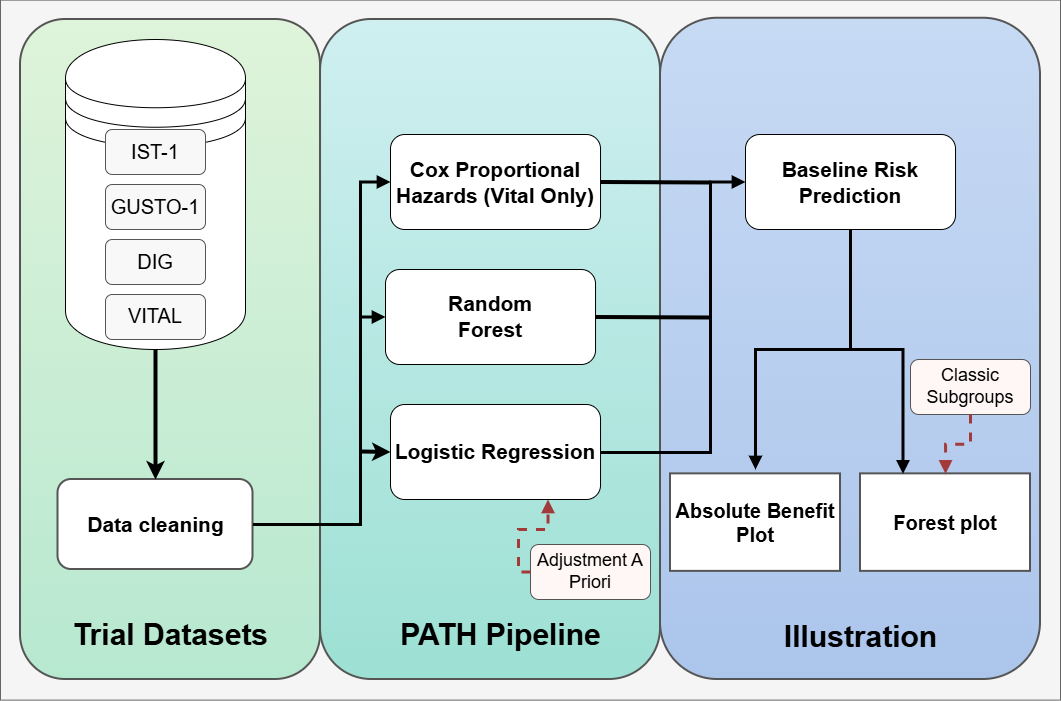
\includegraphics[width=0.8\linewidth]{PATH} 

}

\caption{Overview of the empirical PATH workflow used across the trial analyses.}\label{fig:path-workflow}
\end{figure}

Binary Logistic Regression and Random Forest models were employed for
baseline risk stratification in the GUSTO-I and IST-I trials, with model
specification determined by previously published analyses of the trials.
For the DIG binary outcome analysis, baseline risk stratification was
illustrated using multivariable logistic regression only.

\subsection{GUSTO-I}\label{gusto-i}

For the GUSTO-I trial, baseline risk stratification was performed using
logistic regression and random forest models. Model specification was
adapted from the prognostic model reported by Steyerberg, Bossuyt, and
Lee (2000) for the GUSTO-I trial and subsequently used in PATH
demonstrations. The logistic regression model estimated 30-day mortality
using treatment assignment (tPA versus streptokinase), age, Killip
class, systolic blood pressure, pulse rate, previous myocardial
infarction, and infarct location, as shown in Equation
\ref{eq:gusto-logistic}.

To account for non-linear associations, systolic blood pressure was
truncated at 120 mmHg using the piecewise linear transformation in
Equation \ref{eq:gusto-sysbp}, while pulse rate was modelled using a
spline term with a knot at 50 beats per minute, consistent with the
original model specification. Predicted probabilities of 30-day
mortality were generated for all participants from the fitted model.

A random forest model was also fitted using age, Killip class, systolic
blood pressure, pulse rate, previous myocardial infarction, infarct
location and sex as predictors. The model was implemented using the
ranger package with 1,000 trees and probability estimation enabled.
Individual-level predicted risks from both models were subsequently
incorporated into the PATH framework for risk-based analyses of
treatment effect heterogeneity.

\begin{equation}
\text{Systolic BP}_{\leq 120,\,i} = \min(\text{Systolic BP}_i, 120)
\label{eq:gusto-sysbp}
\end{equation}

\begin{equation}
\begin{aligned}
\text{logit}\big(P(\text{30-day mortality}_i = 1)\big)
&=
\beta_0
+ \beta_1 \text{tPA treatment}_i
+ \beta_2 \text{Age}_i
+ \beta_3 \text{Killip class}_i \\
&\quad
+ \beta_4 \text{Systolic BP}_{\leq 120,\,i}
+ f(\text{Pulse rate}_i)
+ \beta_5 \text{Previous MI}_i
+ \beta_6 \text{Infarct location}_i
\end{aligned}
\label{eq:gusto-logistic}
\end{equation}

A random forest model was developed using the principal baseline
prognostic variables identified in previous GUSTO-I risk models. The
binary outcome was death at day 30, and baseline risk was modelled using
age, Killip class, systolic blood pressure, pulse, previous myocardial
infarction, myocardial infarction location, and sex. Treatment
assignment was excluded to ensure that predicted probabilities reflected
baseline prognosis independent of treatment ({``An {International
Randomized Trial Comparing Four Thrombolytic Strategies} for {Acute
Myocardial Infarction}''} 1993).

\begin{Shaded}
\begin{Highlighting}[]
\CommentTok{\# rf\_fit0 \textless{}{-} ranger(}
\CommentTok{\#   day30 \textasciitilde{} age + Killip + sysbp + pulse + pmi + miloc + sex,}
\CommentTok{\#   data = gusto,}
\CommentTok{\#   probability = TRUE,}
\CommentTok{\#   num.trees = 1000,}
\CommentTok{\#   seed = 88}
\CommentTok{\# )}
\end{Highlighting}
\end{Shaded}

PATH compatible forest plots, similar to those used for displaying the
results of conventional subgroup analyses (Cuzick 2005), were
constructed using the \texttt{metafor} package to present the relative
effects of the GUSTO-I trial across risk quartiles (Figures
\ref{fig:gusto-relative-effects-logistic} and
\ref{fig:gusto-relative-effects-rf}). Additionally, these forest plots
allow for direct comparison of relative effects (ORs) within strata of
traditional subgroups, namely Sex, Age and the location of any
Myocardial Infarctions. These prognostic variables were selected for
their interpretability for a general audience, as well as being
prognostic of 30 day-mortality in the GUSTO-I trial (Califf et al.
1997). The corresponding absolute-benefit plots are presented in Figures
\ref{fig:gusto-absolute-effects-logistic} and
\ref{fig:gusto-absolute-effects-rf}.

\begin{figure}[!htbp]

{\centering 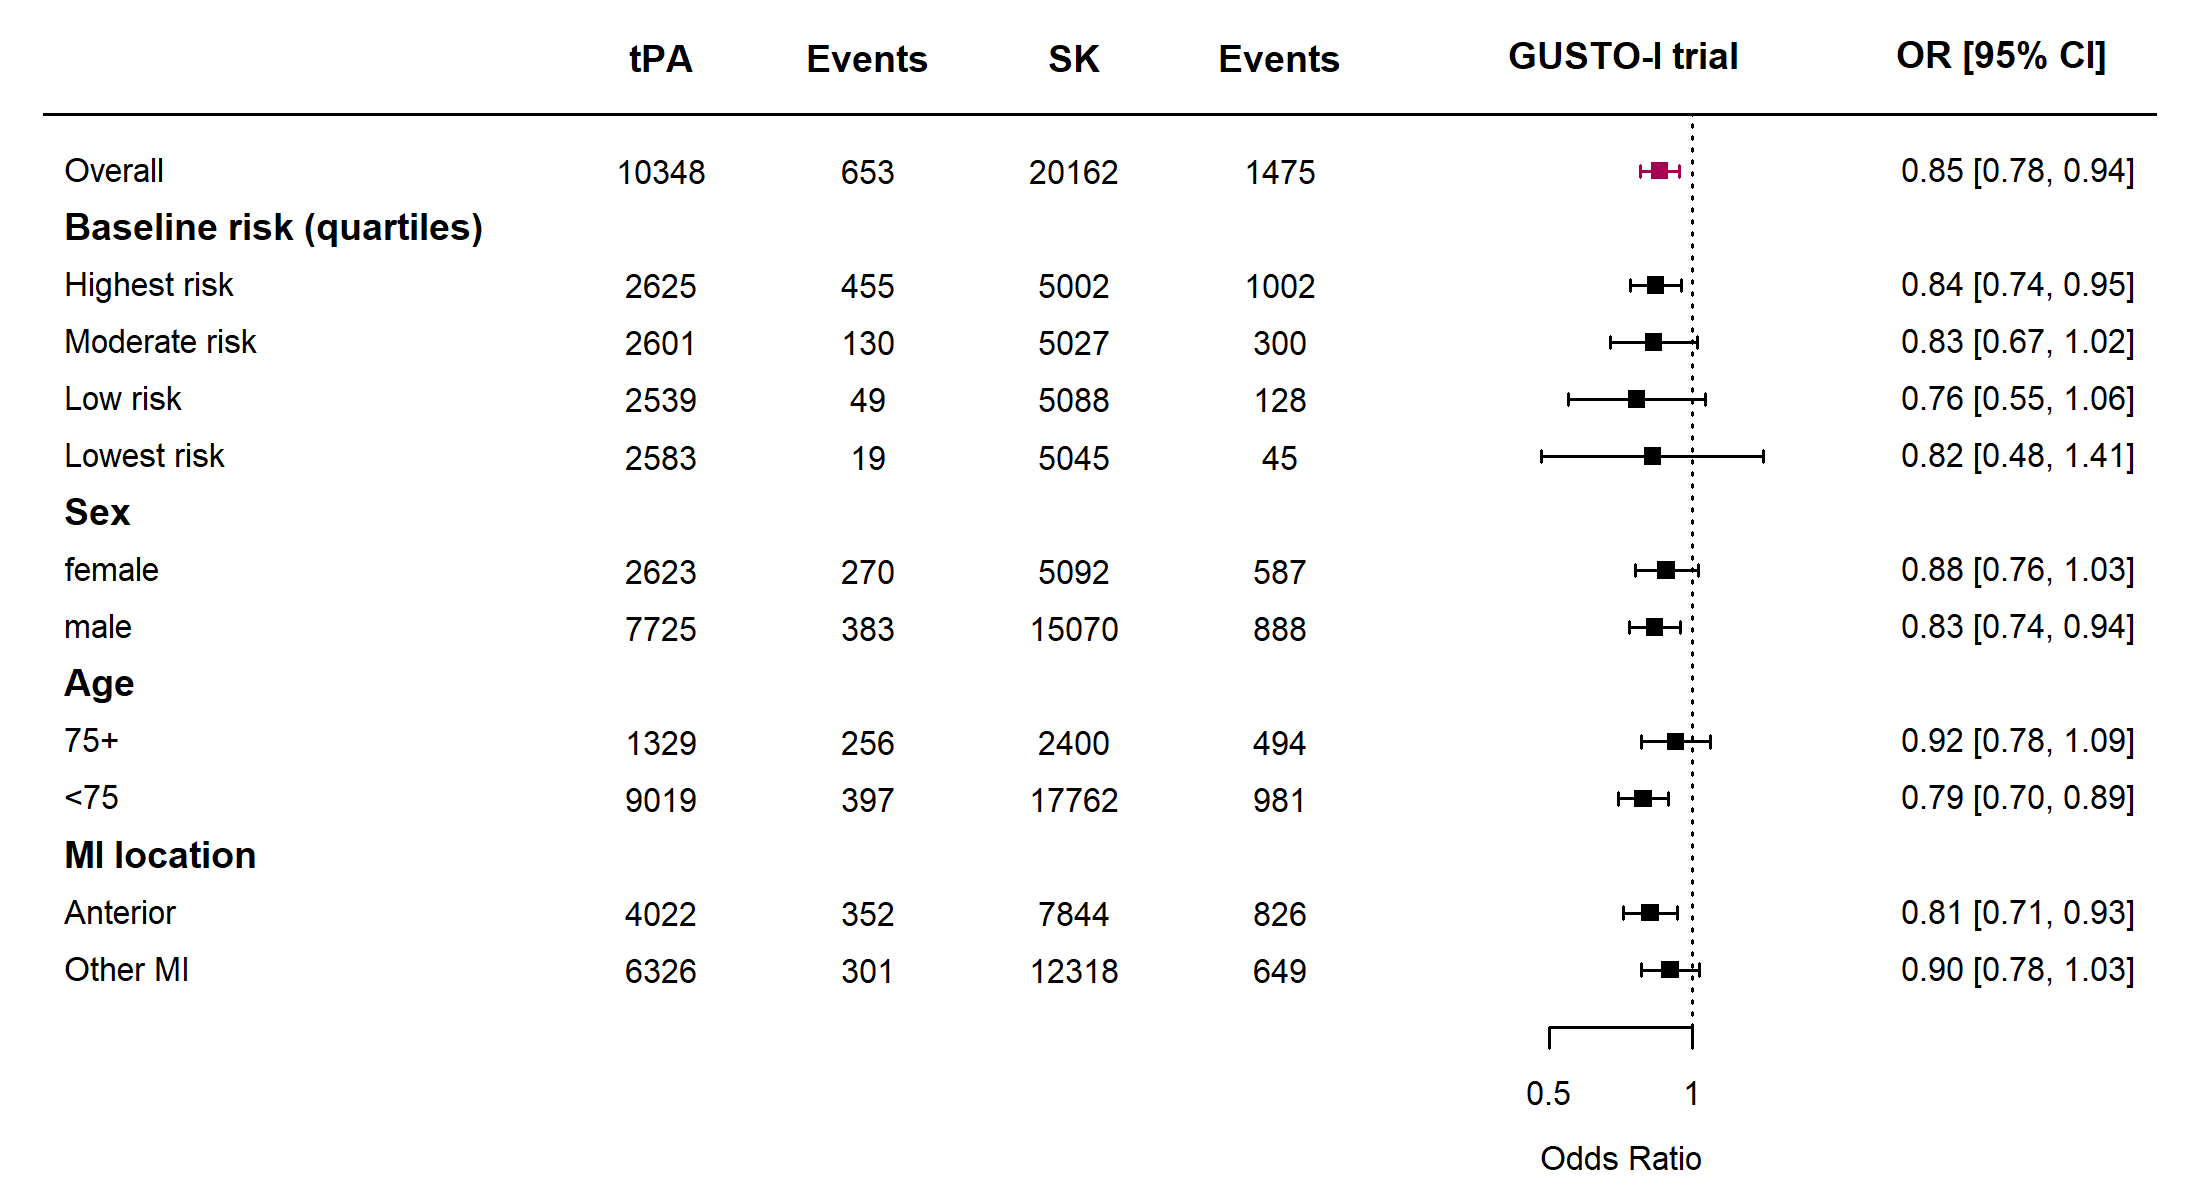
\includegraphics[width=0.95\linewidth]{gusto_report_forest} 

}

\caption{PATH-compatible forest plot showing the relative treatment effect of tissue plasminogen activator compared with streptokinase across baseline-risk quartiles and conventional one-variable-at-a-time subgroups in GUSTO-I, with quartiles derived from the multivariable logistic regression model.}\label{fig:gusto-relative-effects-logistic}
\end{figure}

\begin{figure}[!htbp]

{\centering 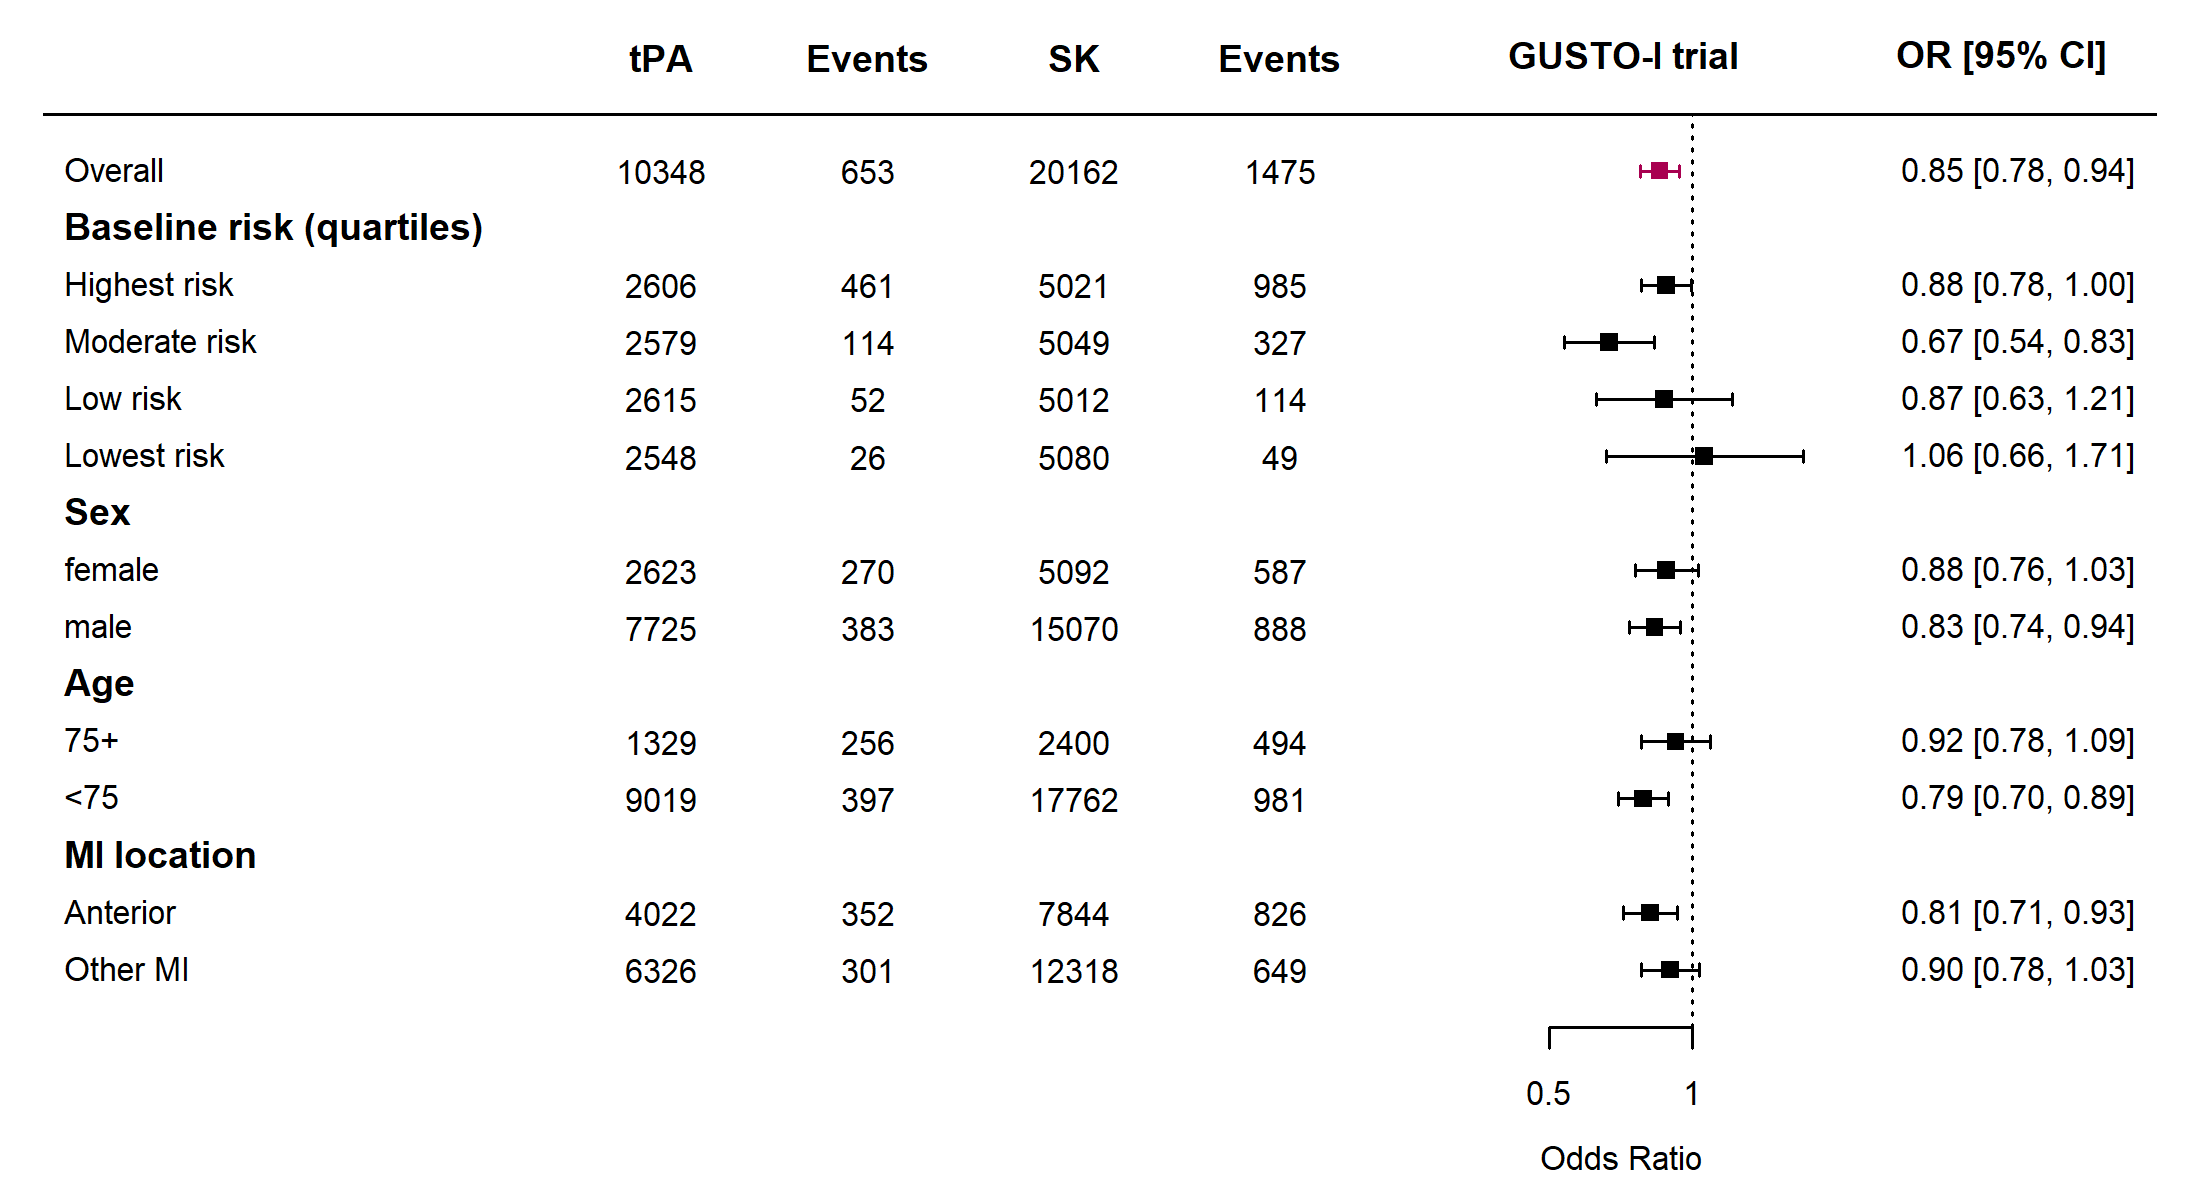
\includegraphics[width=0.95\linewidth]{gusto_rf_report_forest} 

}

\caption{PATH-compatible forest plot showing the relative treatment effect of tissue plasminogen activator compared with streptokinase across baseline-risk quartiles and conventional one-variable-at-a-time subgroups in GUSTO-I, with quartiles derived from the random forest model.}\label{fig:gusto-relative-effects-rf}
\end{figure}

\begin{figure}[!htbp]

{\centering 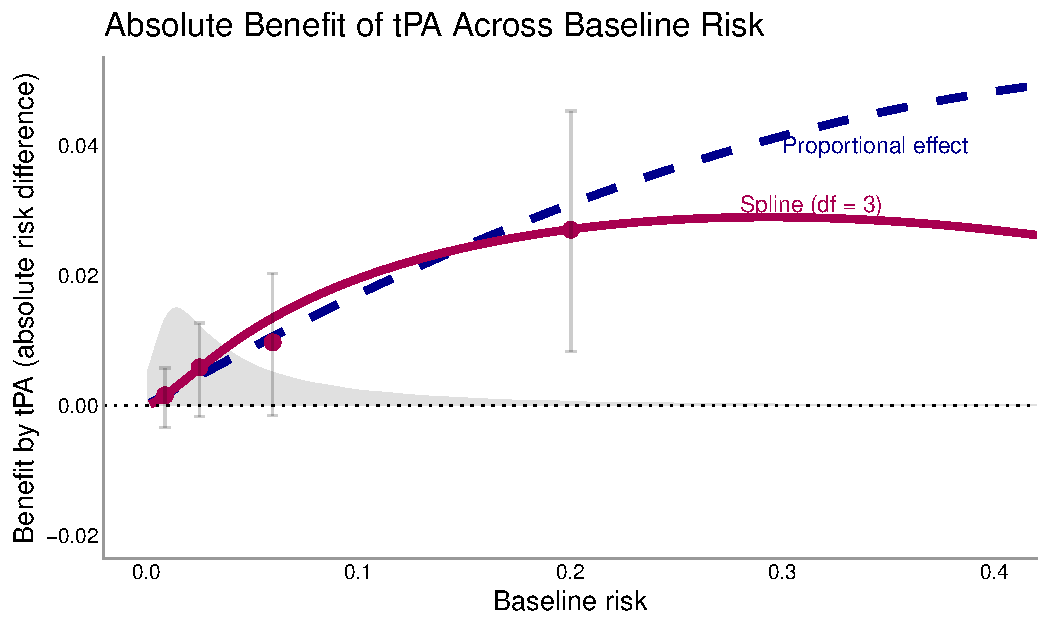
\includegraphics[width=0.88\linewidth]{Methods_files/figure-latex/gusto-absolute-effects-logistic-1} 

}

\caption{Absolute benefit of tissue plasminogen activator compared with streptokinase across predicted baseline risk in GUSTO-I, using the multivariable logistic regression baseline-risk model.}\label{fig:gusto-absolute-effects-logistic}
\end{figure}

\begin{figure}[!htbp]

{\centering 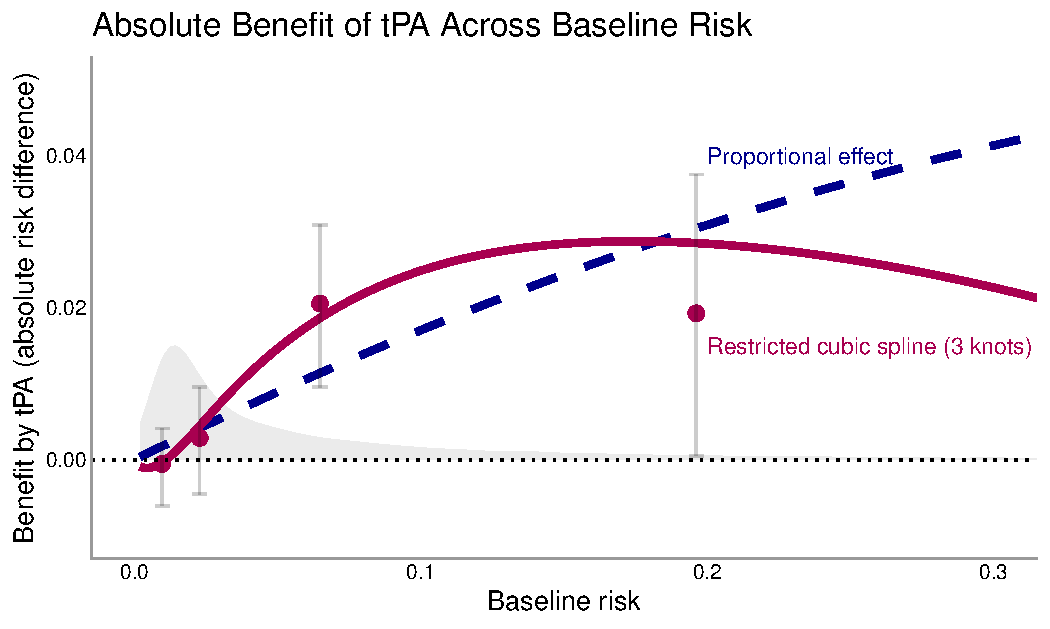
\includegraphics[width=0.88\linewidth]{Methods_files/figure-latex/gusto-absolute-effects-rf-1} 

}

\caption{Absolute benefit of tissue plasminogen activator compared with streptokinase across predicted baseline risk in GUSTO-I, using the random forest baseline-risk model.}\label{fig:gusto-absolute-effects-rf}
\end{figure}

In the GUSTO-I analyses, the PATH-compatible forest plots indicate that
the relative treatment effect of tissue plasminogen activator (tPA),
compared with streptokinase, is broadly maintained across baseline-risk
strata. This supports the interpretation that there is limited
heterogeneity on the relative scale, consistent with the PATH framework
and with the absence of strong evidence for treatment interaction in
relation to baseline risk. However, when the results are viewed on the
absolute scale, heterogeneity becomes more apparent, with patients in
the upper tail of predicted baseline risk deriving greater absolute
benefit from tPA than those at the lower end of the distribution.

The overlaid density plot shows that most patients are concentrated at
relatively low levels of baseline risk, with progressively fewer
patients occupying the upper tail. It is within this smaller higher-risk
subgroup that the estimated treatment benefit becomes most pronounced.
The plots therefore suggest that the main contribution of risk
stratification in GUSTO-I is not to demonstrate major departures from a
proportional relative effect, but rather to show how baseline risk
modifies the absolute clinical value of treatment.

In the logistic regression analyses, the quartile-based estimates appear
more consistent with a proportional effect on the absolute scale,
showing a more orderly increase in benefit as predicted baseline risk
rises. This is in keeping with the smoother absolute-benefit curve,
where benefit increases across risk before flattening in the
highest-risk region. By contrast, the random forest stratification shows
somewhat greater deviation from a simple proportional pattern,
particularly at the extremes of the risk distribution. Together, these
findings suggest that the logistic model yields baseline-risk groupings
that more closely reflect the expected progression from lower to higher
absolute treatment benefit, whereas the random forest captures a less
regular pattern.

\subsection{IST-I}\label{ist-i}

For the IST-I trial, baseline risk stratification was performed using
both logistic regression and random forest models. The logistic
regression model estimated 14-day mortality using age, level of
consciousness, evidence of infarction on computed tomography, motor
deficit severity and atrial fibrillation, as shown in Equation
\ref{eq:ist-logistic}. These variables were selected based on a 2015
study by thompson and colleagues recommending the inclusion of these
covariates for adjustment when performing statistical analyses on the
IST-I trial (Thompson et al. 2015).

\begin{equation}
\begin{aligned}
\text{logit}\big(P(\text{14-day mortality}_i = 1)\big)
&=
\beta_0
+ \beta_1 \text{Age}_i
+ \beta_2 \text{Level of consciousness}_i
+ \beta_3 \text{CT infarction}_i \\
&\quad
+ \beta_4 \text{Motor deficit severity}_i
+ \beta_5 \text{Atrial fibrillation}_i
\end{aligned}
\label{eq:ist-logistic}
\end{equation}

The IST-I logistic model was specified in a deliberately simple form,
including only main effects and no interaction or higher-order terms.
Accordingly, continuous predictors were represented using first-order
linear effects.

A random forest model was also fitted to estimate baseline mortality
risk. Consistent with ensemble-learning approaches previously applied to
the IST dataset in an analysis by Hwangbo and colleagues, all prognostic
baseline variables available prior to treatment allocation were included
as predictors (Hwangbo et al. 2022). These comprised age, sex, level of
consciousness, systolic blood pressure, atrial fibrillation, treatment
delay, sleep status at stroke onset, computed tomography (CT) before
randomization, visible infarction on CT, and various neurological
deficit measures. The model was implemented using the \texttt{ranger}
package with 1,000 trees and probability estimation enabled.
Individual-level predicted risks from both models were subsequently
extracted and risk-based quartiles were constructed for illustration of
the relative treatment effects in Figures
\ref{fig:ist-relative-effects-logistic} and
\ref{fig:ist-relative-effects-rf} and the absolute treatment effects in
Figures \ref{fig:ist-absolute-effects-logistic} and
\ref{fig:ist-absolute-effects-rf}.

\begin{Shaded}
\begin{Highlighting}[]
\CommentTok{\# rf\_fit\_IST \textless{}{-} ranger(}
\CommentTok{\#   death14 \textasciitilde{} AGE + SEX + RCONSC + RSBP + RATRIAL + RDELAY +}
\CommentTok{\#     RSLEEP + RCT + RVISINF + RDEF1 + RDEF2 + RDEF3 + RDEF4 + RDEF5,}
\CommentTok{\#   data = IST\_df,}
\CommentTok{\#   probability = TRUE,}
\CommentTok{\#   num.trees = 1000,}
\CommentTok{\#   seed = 88}
\CommentTok{\# )}
\end{Highlighting}
\end{Shaded}

\begin{figure}[!htbp]

{\centering 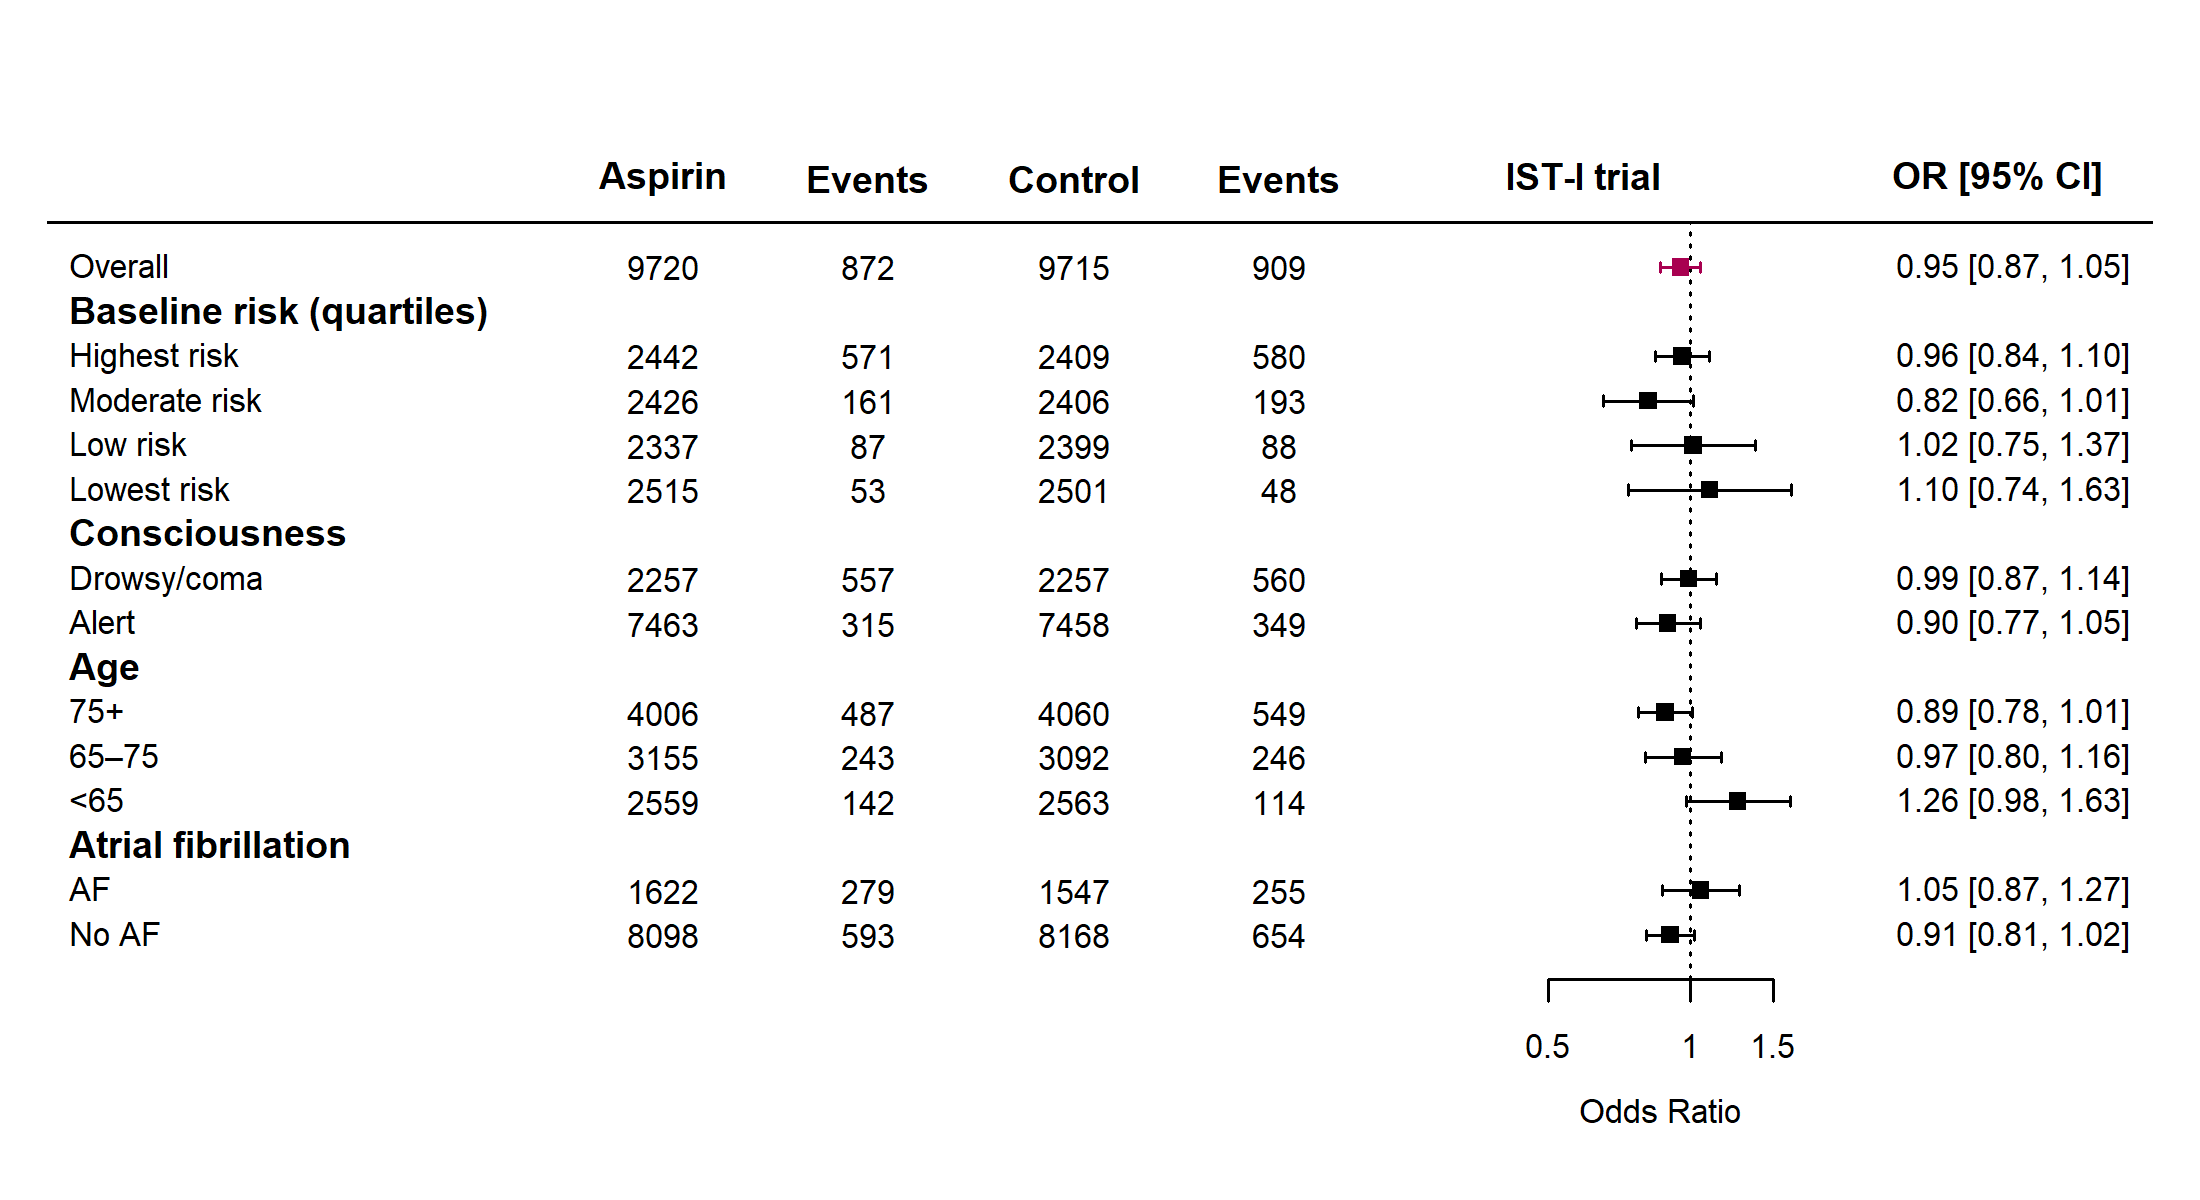
\includegraphics[width=0.95\linewidth]{IST_forest_report} 

}

\caption{PATH-compatible forest plot showing the relative treatment effect of aspirin compared with control across baseline-risk quartiles and conventional one-variable-at-a-time subgroups in IST-I, with quartiles derived from the logistic regression baseline-risk model.}\label{fig:ist-relative-effects-logistic}
\end{figure}

\begin{figure}[!htbp]

{\centering 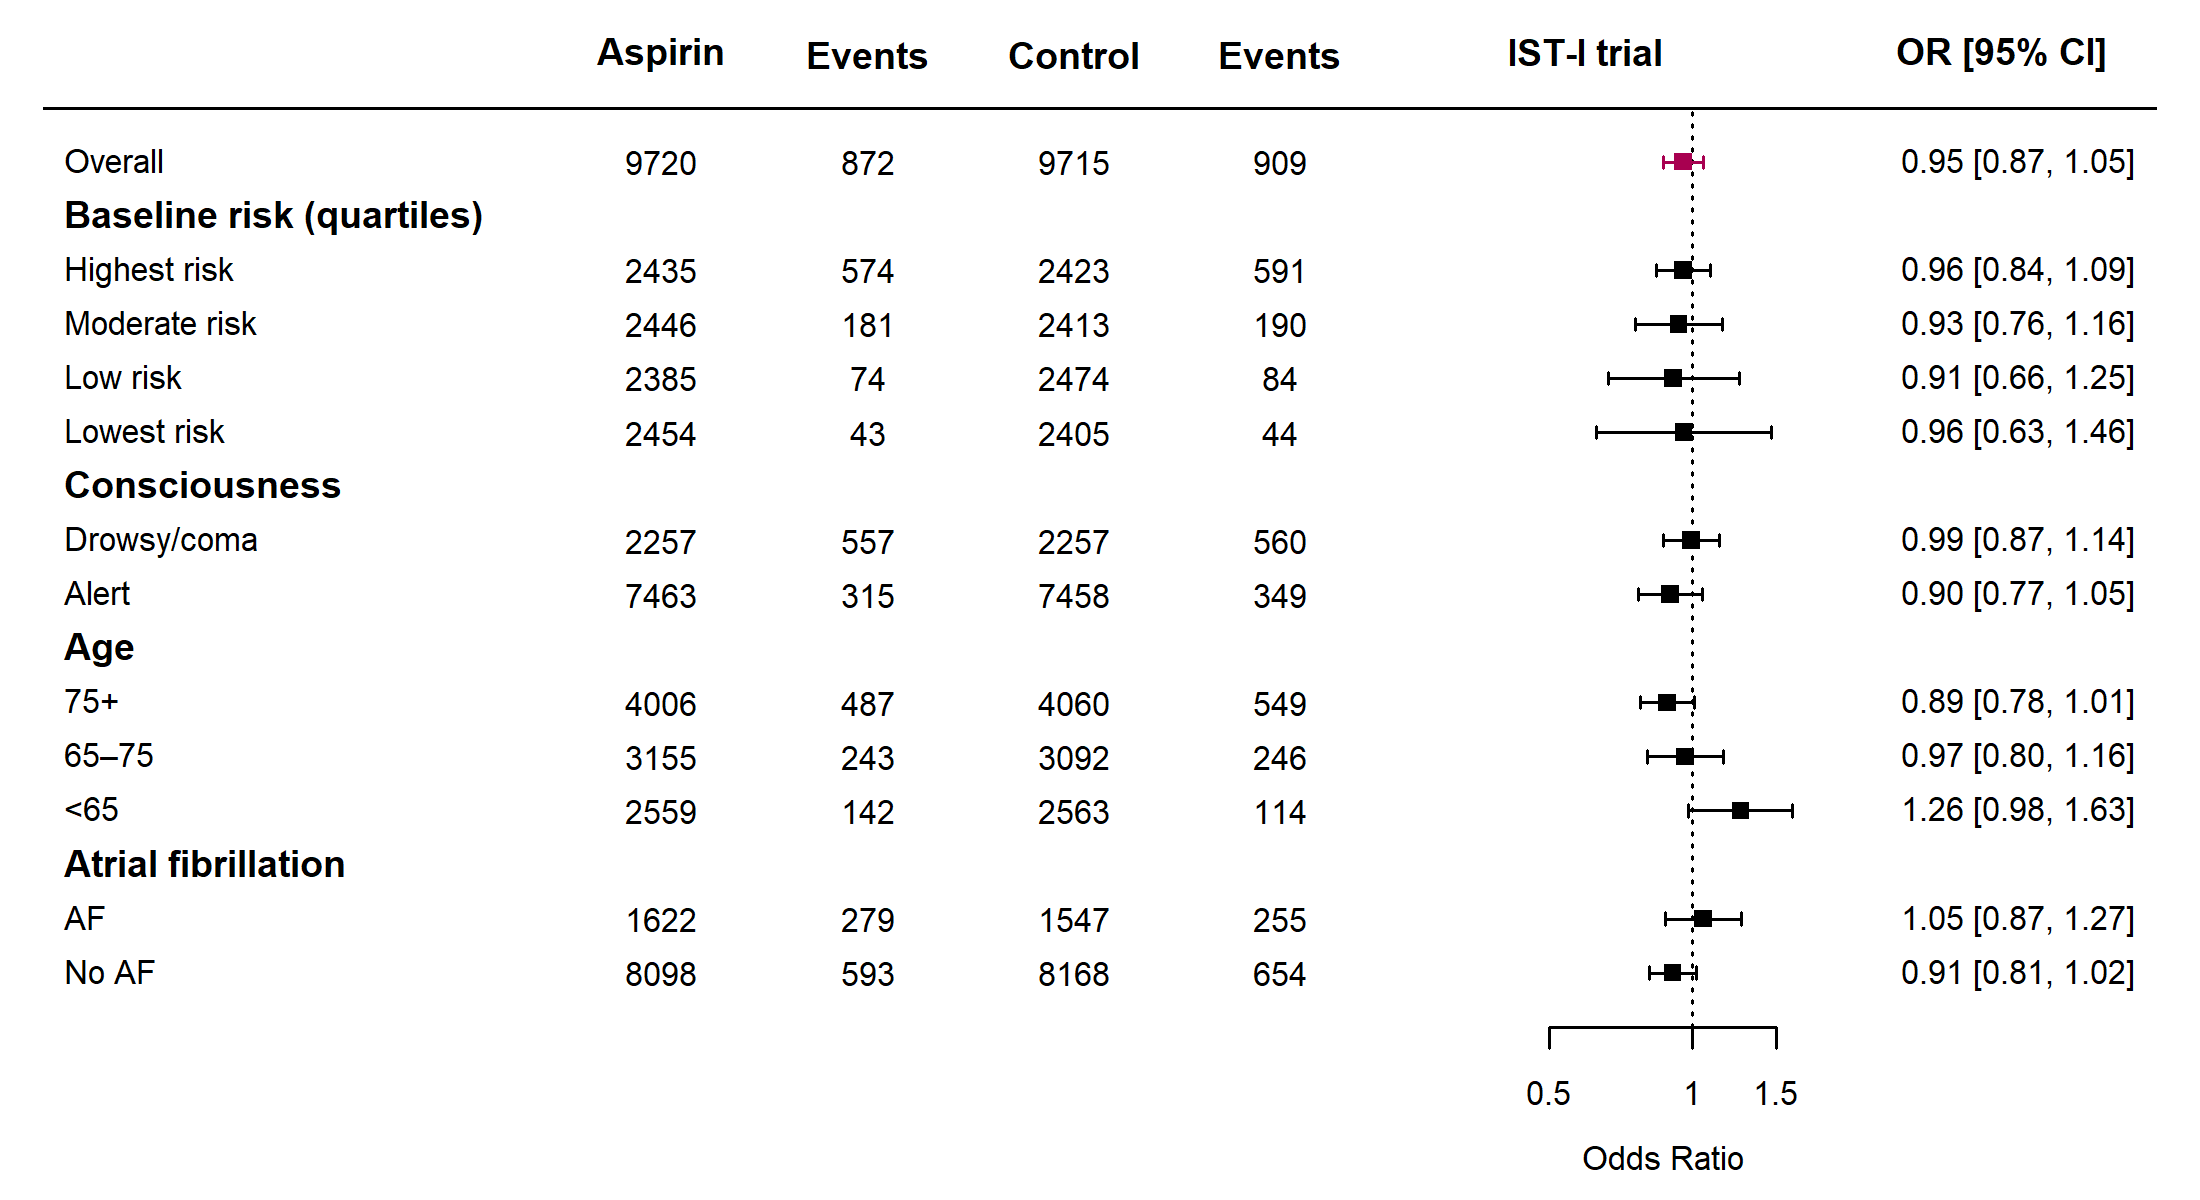
\includegraphics[width=0.95\linewidth]{IST_rf_forest_report} 

}

\caption{PATH-compatible forest plot showing the relative treatment effect of aspirin compared with control across baseline-risk quartiles and conventional one-variable-at-a-time subgroups in IST-I, with quartiles derived from the random forest baseline-risk model.}\label{fig:ist-relative-effects-rf}
\end{figure}

\begin{figure}[!htbp]

{\centering 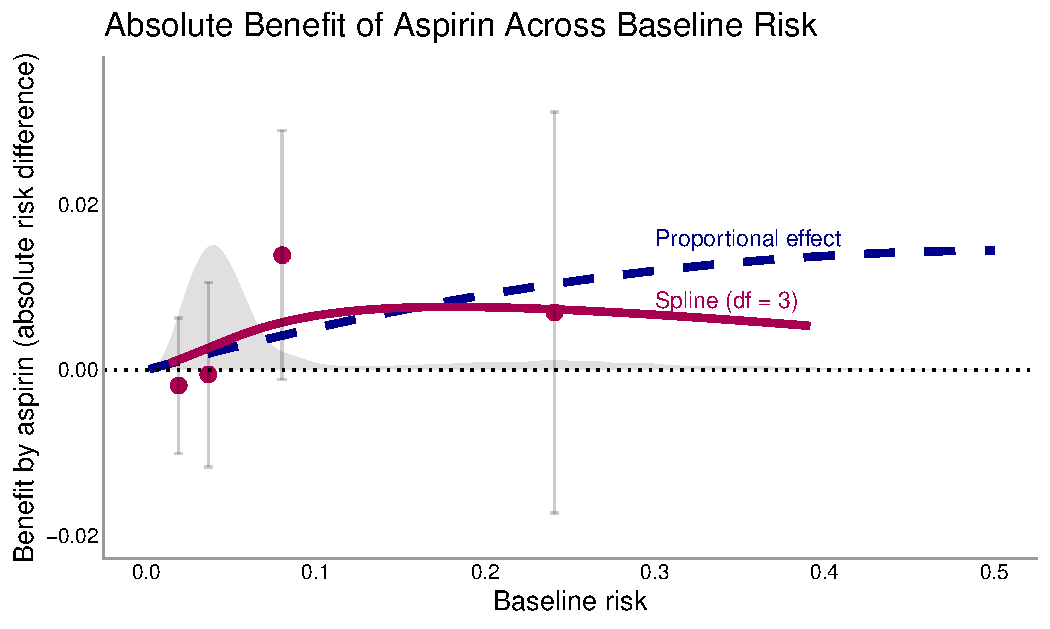
\includegraphics[width=0.88\linewidth]{Methods_files/figure-latex/ist-absolute-effects-logistic-1} 

}

\caption{Absolute benefit of aspirin across predicted baseline risk in IST-I, using the logistic regression baseline-risk model.}\label{fig:ist-absolute-effects-logistic}
\end{figure}

\begin{figure}[!htbp]

{\centering 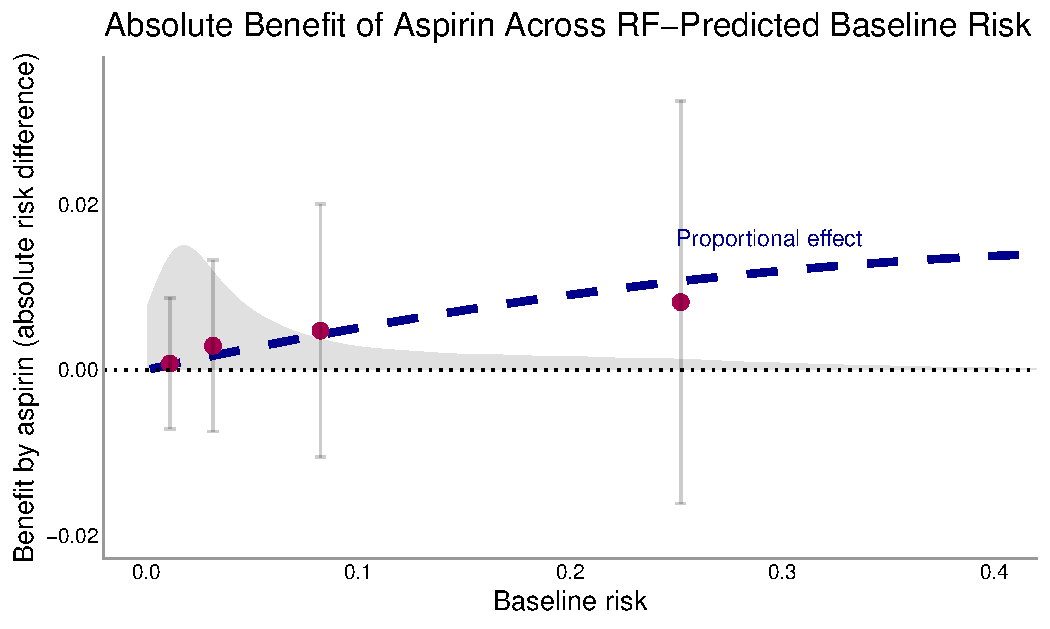
\includegraphics[width=0.88\linewidth]{Methods_files/figure-latex/ist-absolute-effects-rf-1} 

}

\caption{Absolute benefit of aspirin across predicted baseline risk in IST-I, using the random forest baseline-risk model.}\label{fig:ist-absolute-effects-rf}
\end{figure}

In the IST-I analyses, the PATH-compatible forest plots suggest that the
relative treatment effect of aspirin remains broadly consistent across
both baseline-risk quartiles and traditional one-variable-at-a-time
subgroups. The overall odds ratio is close to the null, and the
quartile-specific estimates from both the logistic regression and random
forest baseline-risk models show no clear or consistent departure from
this trial average. Similarly, the estimates across consciousness, age,
and atrial fibrillation subgroups remain largely compatible with a
common relative effect, with confidence intervals overlapping and
generally crossing 1. This supports the interpretation that there is
limited evidence of heterogeneity on the relative scale.

The absolute-benefit plots provide some suggestion that the clinical
effect of aspirin may increase as predicted baseline risk rises,
particularly toward the upper end of the risk distribution. This is
consistent with the PATH framework, where even a relatively stable
proportional effect can translate into larger absolute benefit among
patients at higher underlying risk. However, the grouped estimates are
imprecise, with wide confidence intervals crossing zero across the risk
strata. The evidence for absolute-scale heterogeneity is therefore
suggestive rather than definitive. The Random Forest and logistic
regression models diverge in terms of how they construct the final
baseline risk quartiles. The Random forest model produces quartiles
which almost exactly follow a proportional model, whereas the logistic
regression model produces quartiles which follow a more flexible path.

Overall, there is some indication that higher-risk patients may
experience greater absolute benefit from aspirin, but this pattern is
not statistically significant. This aligns with the overall trial result
shown in the forest plots, where aspirin is associated with a modest
average treatment effect that does not clearly exclude the null.

\subsection{DIG}\label{dig}

For the DIG trial, baseline risk stratification was performed using
logistic regression. The logistic regression model estimated all-cause
mortality using age, New York Heart Association (NYHA) functional class,
systolic blood pressure, previous myocardial infarction, and left
ventricular ejection fraction, as shown in Equation
\ref{eq:dig-logistic}. Predictor selection was informed by established
prognostic factors identified in analyses of the Digitalis Investigation
Group trial and subsequent investigations of mortality risk among
patients with heart failure and preserved systolic function in the DIG
cohort ({``An {International Randomized Trial Comparing Four
Thrombolytic Strategies} for {Acute Myocardial Infarction}''} 1993;
Jones, Francis, and Lauer 2004).

\begin{equation}
\begin{aligned}
\text{logit}\big(P(\text{All-cause mortality}_i = 1)\big)
&=
\beta_0
+ \beta_1 \text{Age}_i
+ \beta_2 \text{NYHA class}_i
+ \beta_3 \text{Systolic blood pressure}_i \\
&\quad
+ \beta_4 \text{Previous MI}_i
+ \beta_5 \text{Left ventricular ejection fraction}_i
\end{aligned}
\label{eq:dig-logistic}
\end{equation}

\begin{figure}[!htbp]

{\centering 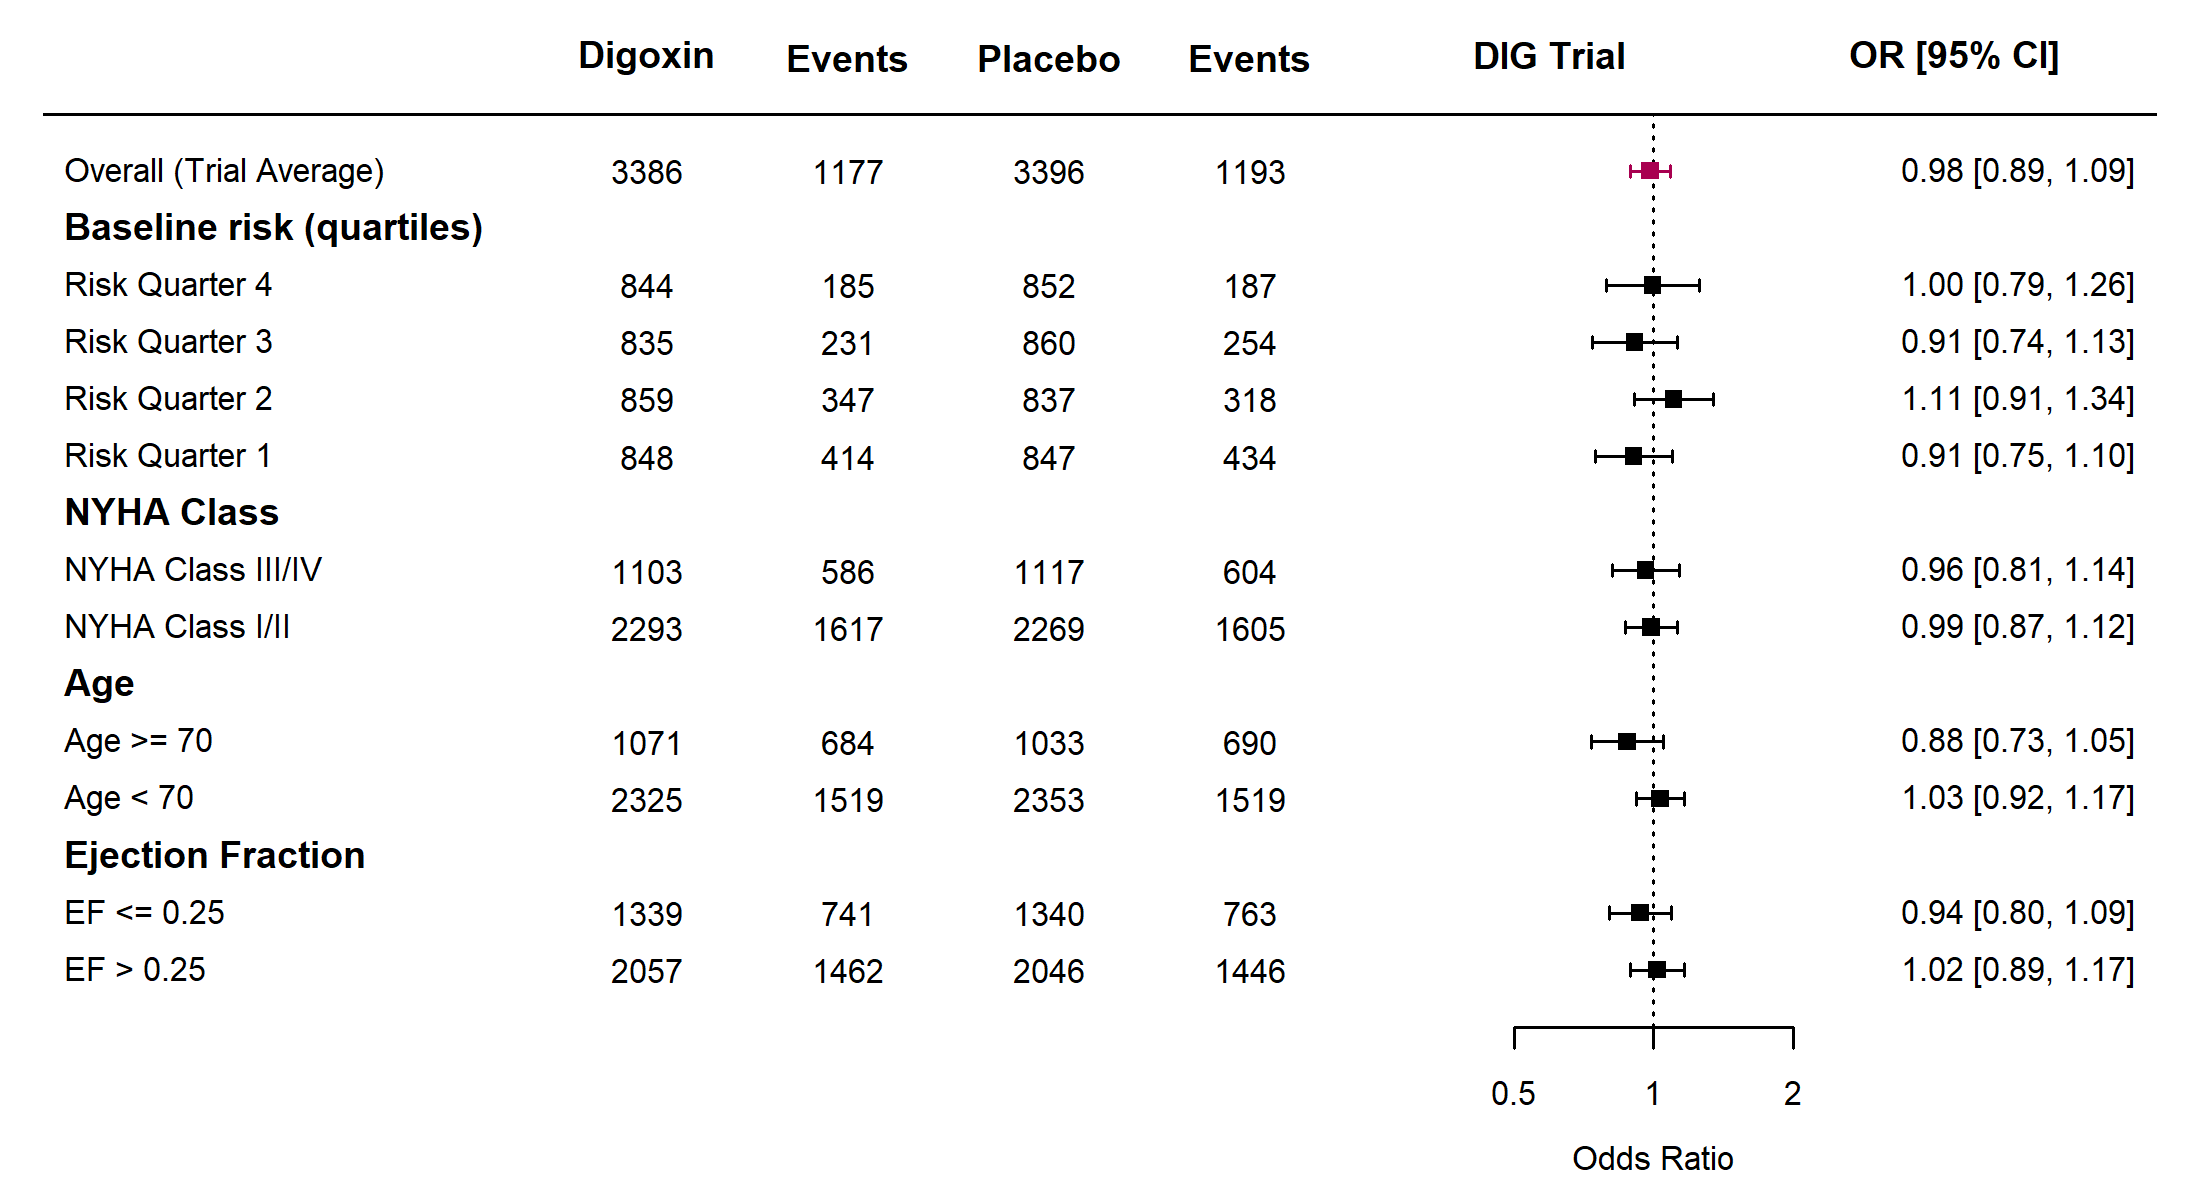
\includegraphics[width=0.95\linewidth]{DIG_report_forest} 

}

\caption{PATH-compatible forest plot showing the relative treatment effect of digoxin compared with placebo across baseline-risk quartiles and conventional one-variable-at-a-time subgroups in the DIG trial.}\label{fig:dig-relative-effect}
\end{figure}

\begin{figure}[!htbp]

{\centering 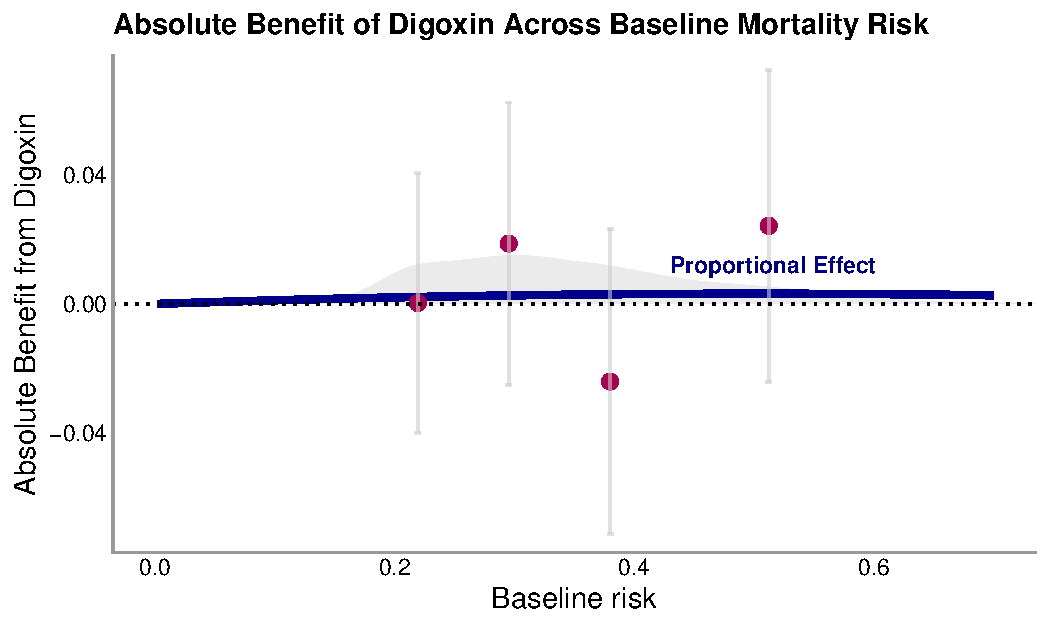
\includegraphics[width=0.88\linewidth]{Methods_files/figure-latex/dig-absolute-effect-1} 

}

\caption{Absolute benefit of digoxin across predicted baseline mortality risk in the DIG trial.}\label{fig:dig-absolute-effect}
\end{figure}

In the DIG analysis, there is little evidence of heterogeneity in either
the relative or absolute treatment effect of digoxin compared with
placebo. The PATH-compatible forest plot in Figure
\ref{fig:dig-relative-effect} shows an overall trial estimate close to
the null, with an odds ratio of 0.98, and the risk-based quartiles do
not show a consistent departure from this overall effect. The
quartile-specific estimates fluctuate around the line of no effect, with
confidence intervals crossing 1 throughout, suggesting no clear evidence
that the relative effect of digoxin differs across the distribution of
predicted baseline mortality risk.

The absolute-benefit plot in Figure \ref{fig:dig-absolute-effect}
reaffirms this. Across the distribution of baseline risk of mortality,
the estimated benefit remains close to zero, and the proportional-effect
curve is essentially flat. Although the observed quartile estimates vary
slightly above and below the null, the uncertainty around these
estimates is substantial. The overlaid density plot shows where patients
are concentrated along the baseline-risk distribution, but unlike GUSTO,
movement into higher-risk regions does not translate into a clearer
absolute treatment benefit.

This result is useful as a control case for the PATH approach. The DIG
trial did not demonstrate a meaningful overall effect of digoxin on
mortality, so there is limited reason to expect risk-based
stratification to reveal clinically important treatment-effect
heterogeneity. In addition, because the DIG training dataset involved
permuted variables, the ability to detect genuine heterogeneity may be
further limited by the structure of the available data. For this reason,
the DIG binary outcome analysis was illustrated using the multivariable
logistic-regression model only, rather than extending the analysis to a
random forest model where there was little underlying treatment signal.

\subsection{VITAL}\label{vital}

For the VITAL trial, baseline risk stratification was performed using a
Cox proportional hazards model rather than logistic regression or random
forest. The model estimated 5-year risk of cardiovascular death using
age, body mass index, sex, use of antihypertensive medication, diabetes
status, current smoking status, and family history of myocardial
infarction, as shown in Equation \ref{eq:vital-cox}. A 5-year time
horizon was selected because the median follow-up in VITAL was 5.3
years, providing a cutoff that retained a large proportion of the
available patient data while still allowing sufficient time for recorded
cardiovascular events to accrue. Covariate selection was informed by the
adjusted VITAL cohort analysis reported by Caldeira et al. (2023),
reflecting baseline demographic and cardiovascular risk characteristics
available prior to treatment allocation.

\begin{equation}
\begin{aligned}
h(t \mid X_i)
&=
h_0(t)\exp\Big(
\beta_1 \text{Age}_i
+ \beta_2 \text{Body mass index}_i
+ \beta_3 \text{Sex}_i \\
&\quad
+ \beta_4 \text{Antihypertensive medication}_i
+ \beta_5 \text{Current smoking}_i \\
&\quad
+ \beta_6 \text{Diabetes}_i
+ \beta_7 \text{Family history of MI}_i
\Big)
\end{aligned}
\label{eq:vital-cox}
\end{equation}

For prediction, the baseline survival function was estimated from the
fitted \texttt{coxph} model using \texttt{survfit}, and then evaluated
at \(t = 5\) years. Writing the linear predictor as
\(\eta_i = \beta_1 \text{Age}_i + \beta_2 \text{Body mass index}_i + \beta_3 \text{Sex}_i + \beta_4 \text{Antihypertensive medication}_i + \beta_5 \text{Current smoking}_i + \beta_6 \text{Diabetes}_i + \beta_7 \text{Family history of MI}_i\),
the corresponding survival function is obtained as

\begin{equation}
H(t \mid X_i)
=
\int_0^t h(u \mid X_i)\,du
=
\exp(\eta_i)\int_0^t h_0(u)\,du
=
\exp(\eta_i)H_0(t),
\end{equation}

\begin{equation}
S(t \mid X_i)
=
\exp\big(-H(t \mid X_i)\big)
=
\exp\big(-H_0(t)\exp(\eta_i)\big)
=
\big[S_0(t)\big]^{\exp(\eta_i)},
\end{equation}

where \(S_0(t)=\exp\{-H_0(t)\}\) is the baseline survival function.
Accordingly, individual 5-year risk was obtained as
\(1 - S(5 \mid X_i)\).

\begin{figure}[!htbp]

{\centering 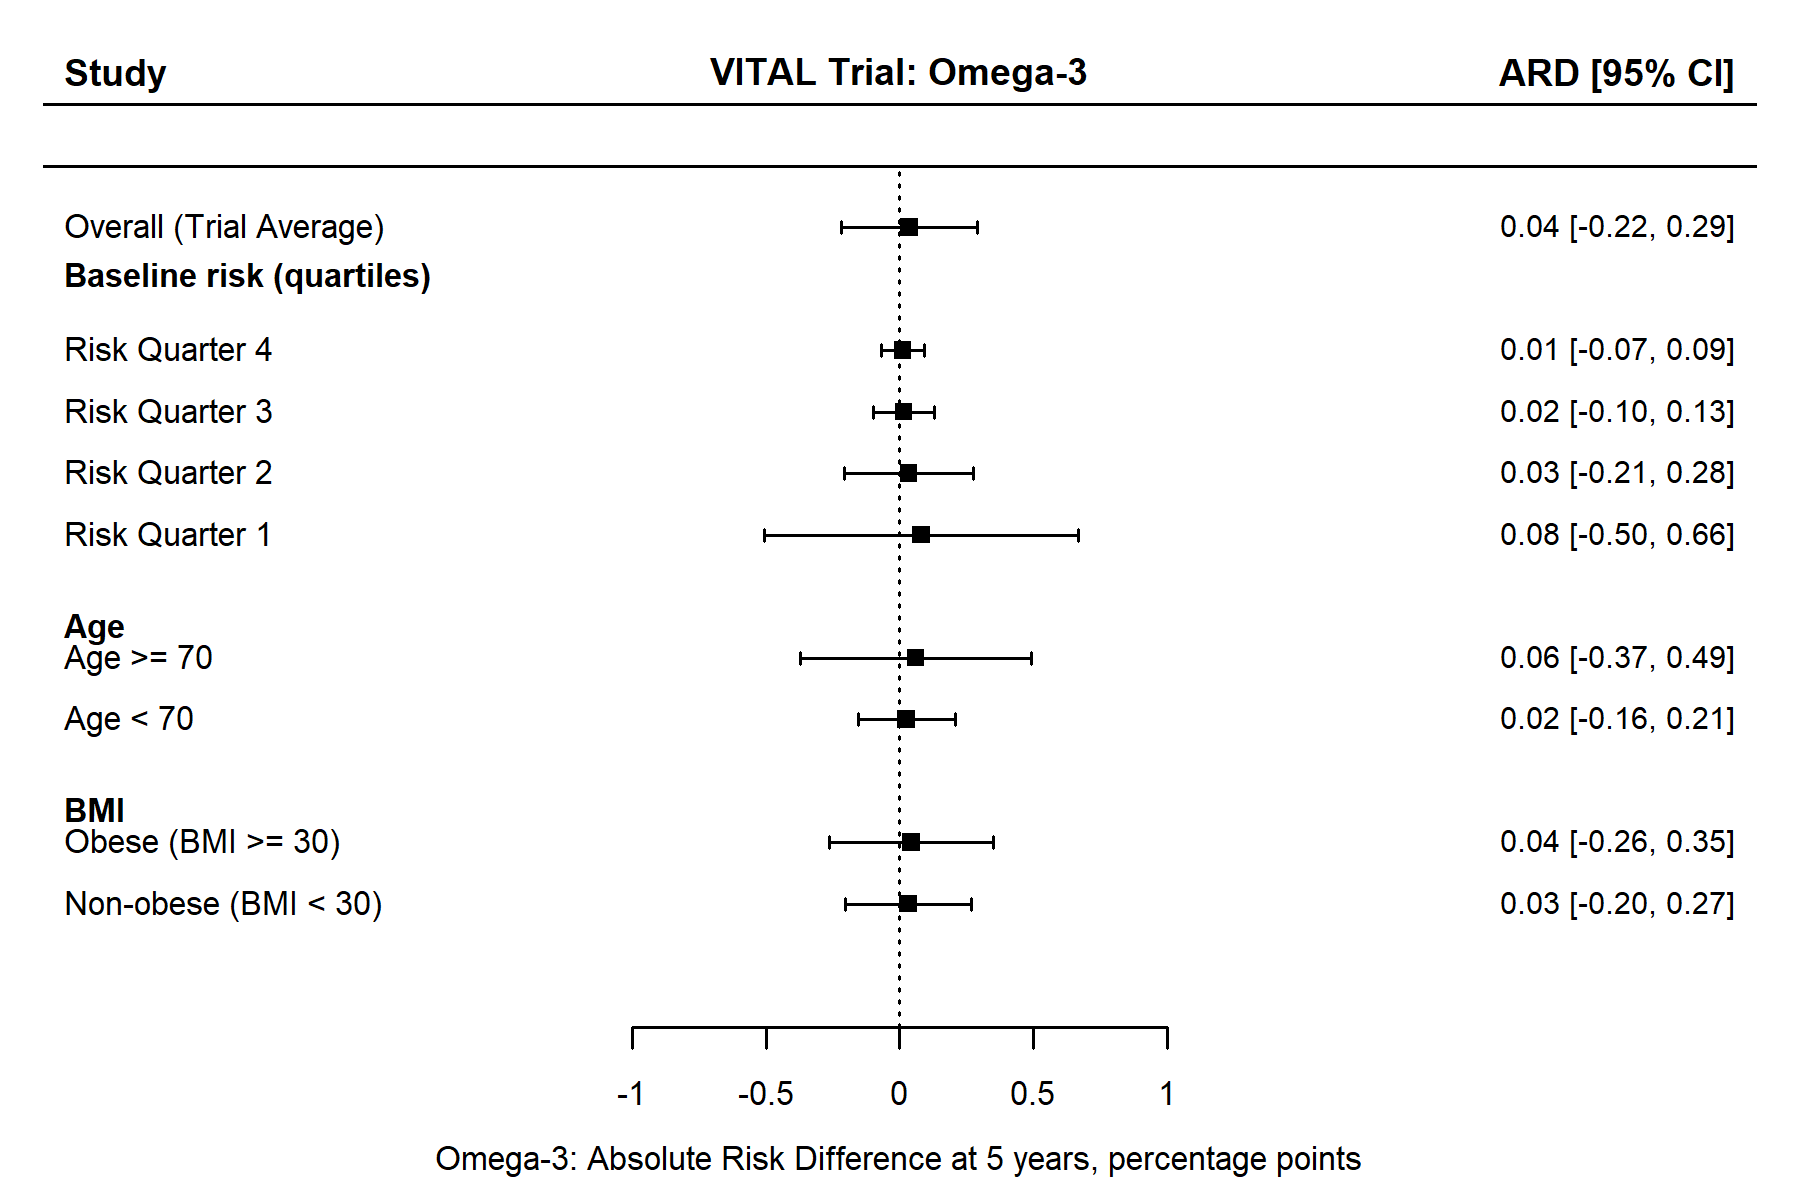
\includegraphics[width=0.95\linewidth]{VITAL_report_forest_omega} 

}

\caption{PATH-compatible forest plot showing absolute risk differences for omega-3 supplementation across baseline-risk quartiles and conventional subgroups in VITAL.}\label{fig:vital-relative-effects-omega}
\end{figure}

\begin{figure}[!htbp]

{\centering 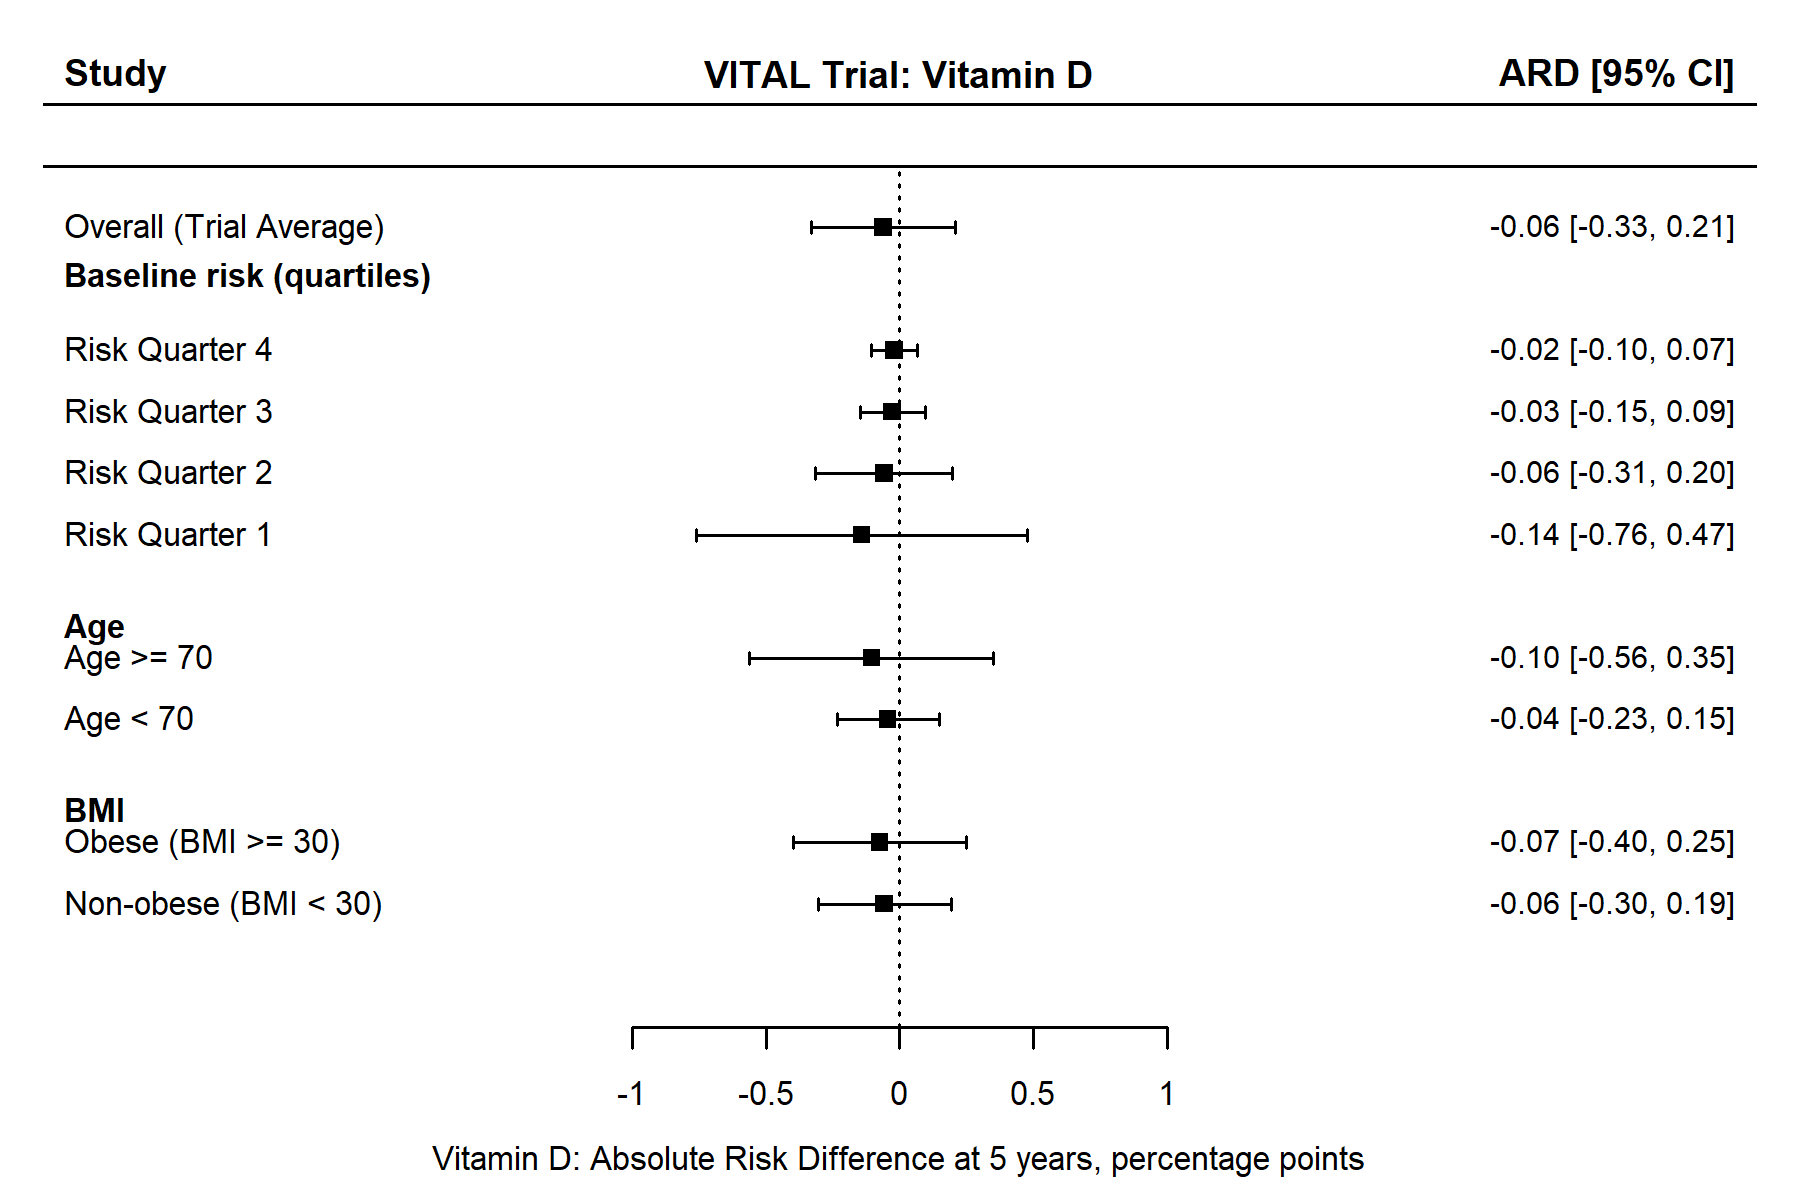
\includegraphics[width=0.95\linewidth]{VITAL_report_forest_vitd} 

}

\caption{PATH-compatible forest plot showing absolute risk differences for vitamin D supplementation across baseline-risk quartiles and conventional subgroups in VITAL.}\label{fig:vital-relative-effects-vitd}
\end{figure}

\begin{figure}[!htbp]

{\centering 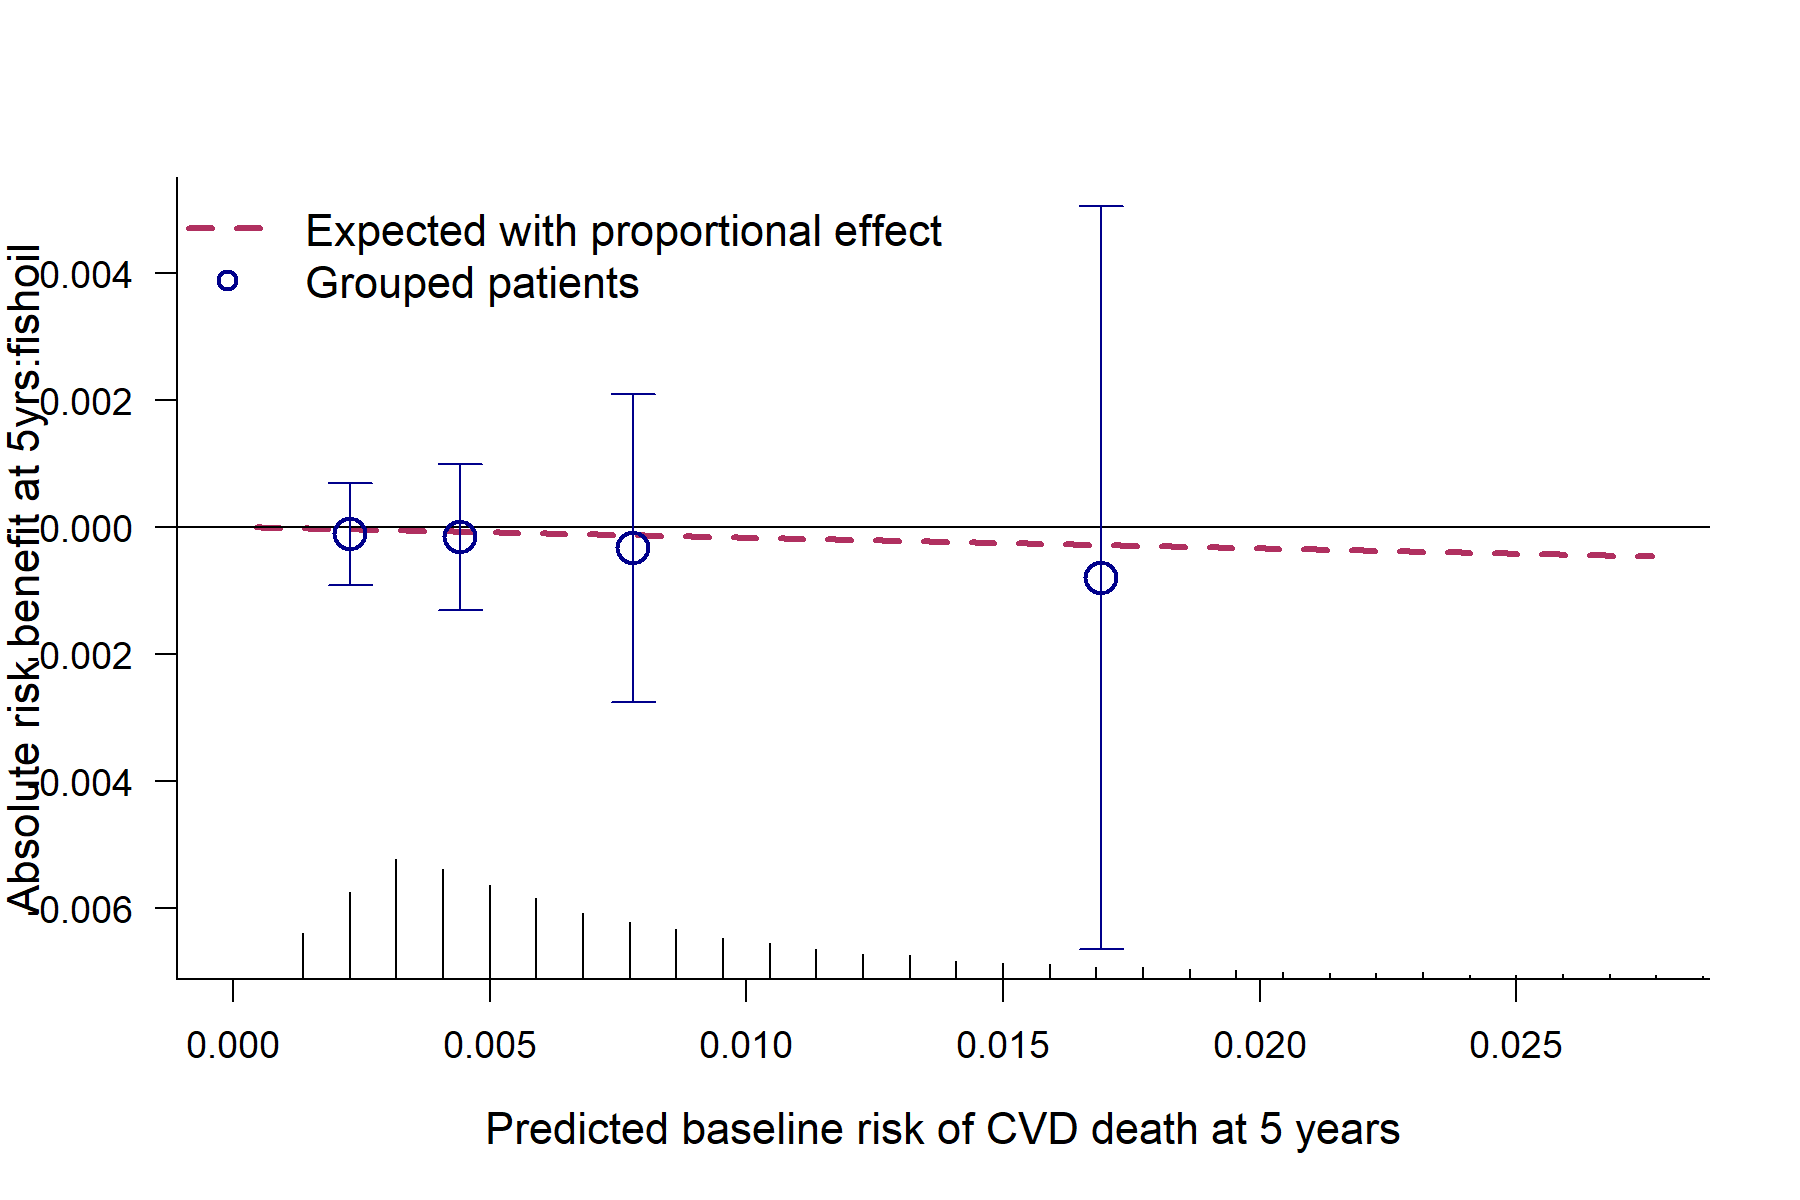
\includegraphics[width=0.88\linewidth]{VITAL_plot_omg} 

}

\caption{Absolute benefit of omega-3 supplementation across predicted 5-year baseline risk of cardiovascular death in VITAL.}\label{fig:vital-absolute-effects-omega}
\end{figure}

\begin{figure}[!htbp]

{\centering 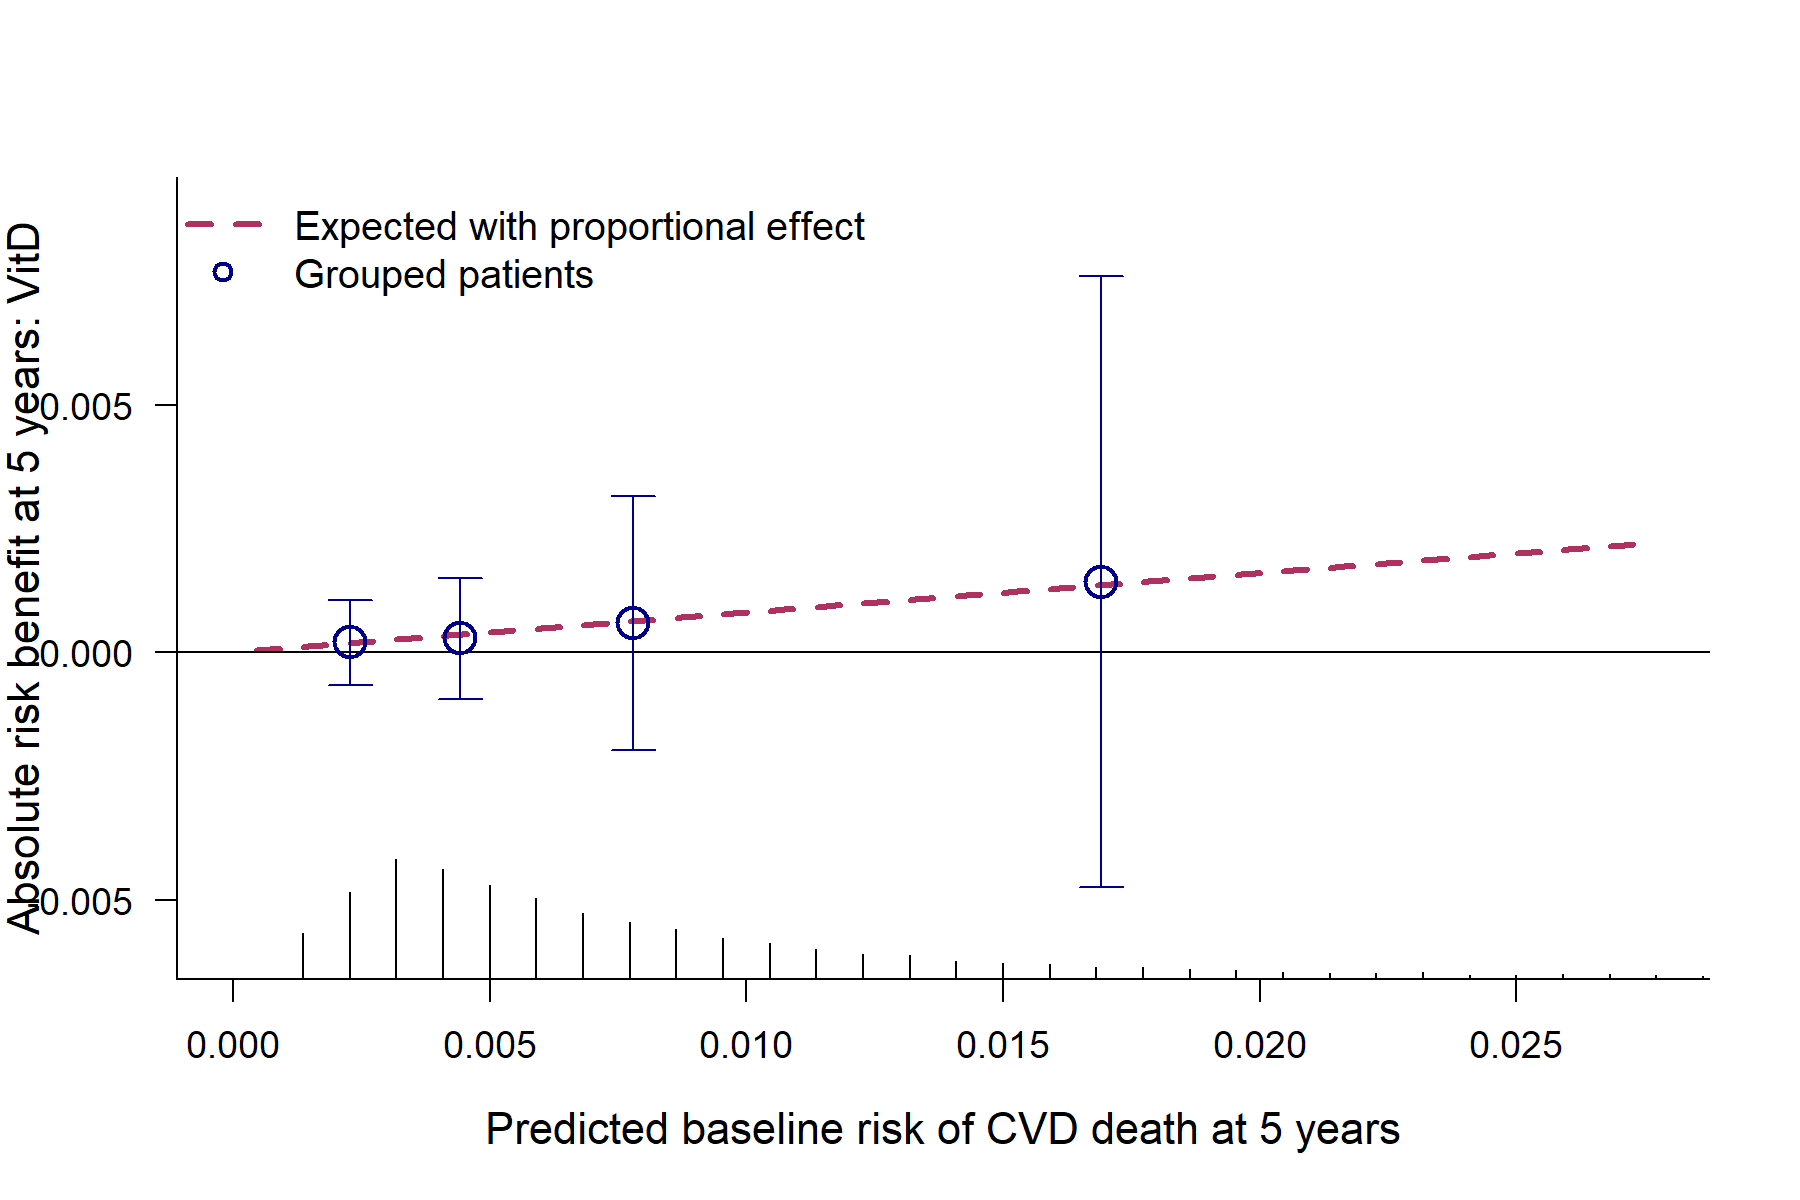
\includegraphics[width=0.88\linewidth]{VITAL_plot_Vit} 

}

\caption{Absolute benefit of vitamin D supplementation across predicted 5-year baseline risk of cardiovascular death in VITAL.}\label{fig:vital-absolute-effects-vitd}
\end{figure}

The VITAL analysis required a different modelling approach from the
binary outcome trials because the endpoint was time to cardiovascular
death at 5 years, rather than a fixed-date, binary outcome. Baseline
risk was therefore estimated using the Cox proportional hazards model in
Equation \ref{eq:vital-cox}, with covariates selected from the adjusted
VITAL cohort analysis by Caldeira and colleagues (Caldeira et al. 2023).
The trial itself also had a more challenging structure than the others,
using a 2-by-2 factorial design to evaluate vitamin D supplementation
and marine omega-3 fatty acid supplementation within the same study
population. For the PATH analysis, this meant that absolute risk
differences were estimated separately for each intervention, while still
employing the same PATH workflow.

Across both the omega-3 and vitamin D analyses, there is little evidence
of treatment-effect heterogeneity. The PATH-compatible forest plots in
Figures \ref{fig:vital-relative-effects-omega} and
\ref{fig:vital-relative-effects-vitd} show overall absolute risk
differences close to zero, and the risk-based quartiles do not show a
consistent departure from the trial average. The subgroup estimates by
age and BMI also remain close to the null, with confidence intervals
crossing zero throughout. This result aligns with the overall reported
findings from VITAL, where neither vitamin D nor omega-3 supplementation
demonstrated a clear overall effect on the principal cardiovascular
outcomes.

The absolute-benefit plots in Figures
\ref{fig:vital-absolute-effects-omega} and
\ref{fig:vital-absolute-effects-vitd} support the same interpretation on
the continuous baseline-risk scale. For both vitamin D and omega-3, the
estimated absolute benefit remains very close to zero across the
observed range of baseline risk. The patient distribution is
concentrated at low predicted 5-year risk of cardiovascular death, and
movement into the higher-risk tail does not reveal a clear increase in
absolute benefit. Overall, the VITAL results therefore act as another
example where the absence of a strong overall treatment effect is
reflected in the absence of meaningful risk-based heterogeneity.

\FloatBarrier

\subsection{Monte Carlo simulations}\label{monte-carlo-simulations}

The Monte Carlo simulation study was designed using the ADEMP structure
described by Morris and colleagues in 2019 where simulation studies are
specified according to their Aim, Data-generating mechanism, Estimand,
Methods and Performance measure (Morris, White, and Crowther 2019). The
aim was to assess whether a risk-based interaction test would falsely
detect treatment-effect heterogeneity when no true interaction was
present. This was used as a null simulation to evaluate the Type I error
behaviour of the likelihood ratio test used in the PATH analyses.

\begin{figure}[!htbp]

{\centering 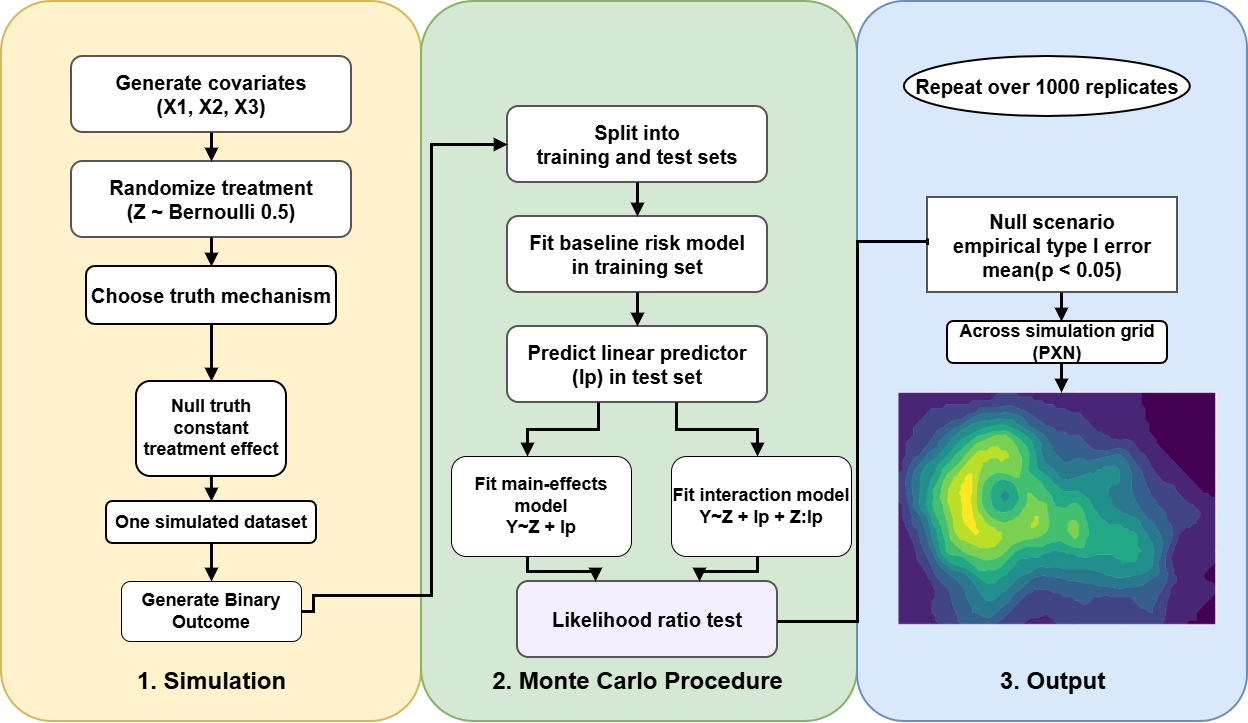
\includegraphics[width=1\linewidth]{MC_FLOW} 

}

\caption{Workflow of the Monte Carlo simulation study used to assess how variation in model dimension and sample size influences empirical Type I error in the null treatment-by-risk interaction setting.}\label{fig:mc-flow}
\end{figure}

For each simulated dataset, \(p\) independent prognostic covariates were
generated from standard normal distributions, such that
\(X_{ij} \sim N(0,1)\) for \(j = 1, \ldots, p\), and treatment
assignment was generated independently with equal probability of
allocation to treatment or control. In the data-generating model, each
prognostic covariate contributed equally to the outcome through a
coefficient of 0.5. Binary outcomes were then generated from the
logistic model in Equation \ref{eq:simulation-outcome}, with a constant
treatment effect and no treatment-by-covariate interaction:

\begin{equation}
\text{logit}\{P(Y_i = 1)\}
=
-2 - 0.5Z_i + 0.5\sum_{j=1}^{p}X_{ij}.
\label{eq:simulation-outcome}
\end{equation}

The simulation varied the sample size across
\(n = 50, 75, 100, 150, 200, 300, 500, 750, 1000, 2000,\) and \(5000\),
and varied the number of prognostic covariates from \(p = 1\) to
\(p = 10\). For each condition, the dataset was split equally into
training and test samples. A logistic baseline risk model was fitted in
the training sample using the prognostic covariates only. The fitted
model was then used to generate a linear predictor in the test sample.

The method compared a null model against an alternative interaction
model in the test sample:

\begin{equation}
H_0:\ \text{logit}\{P(Y_i = 1)\} = \beta_0 + \beta_1 Z_i + \beta_2 lp_i
\label{eq:simulation-main}
\end{equation}

\begin{equation}
H_1:\ \text{logit}\{P(Y_i = 1)\} = \beta_0 + \beta_1 Z_i + \beta_2 lp_i + \beta_3 (Z_i \times lp_i)
\label{eq:simulation-interaction}
\end{equation}

The estimand was the null treatment-by-risk interaction,
\(H_0:\beta_{Z \times lp}=0\). A likelihood ratio test was used to
compare the main-effects model in Equation \ref{eq:simulation-main} with
the interaction model in Equation \ref{eq:simulation-interaction}, and
the performance measure was the empirical Type I error rate, defined as
the proportion of Monte Carlo repetitions with \(p < 0.05\). For each
simulation condition, 1000 Monte Carlo repetitions were performed. The
simulation results were summarised as a Type I error surface across
sample size and number of prognostic parameters (Figure
\ref{fig:mc-type1-surface}).

\begin{figure}[!htbp]

{\centering 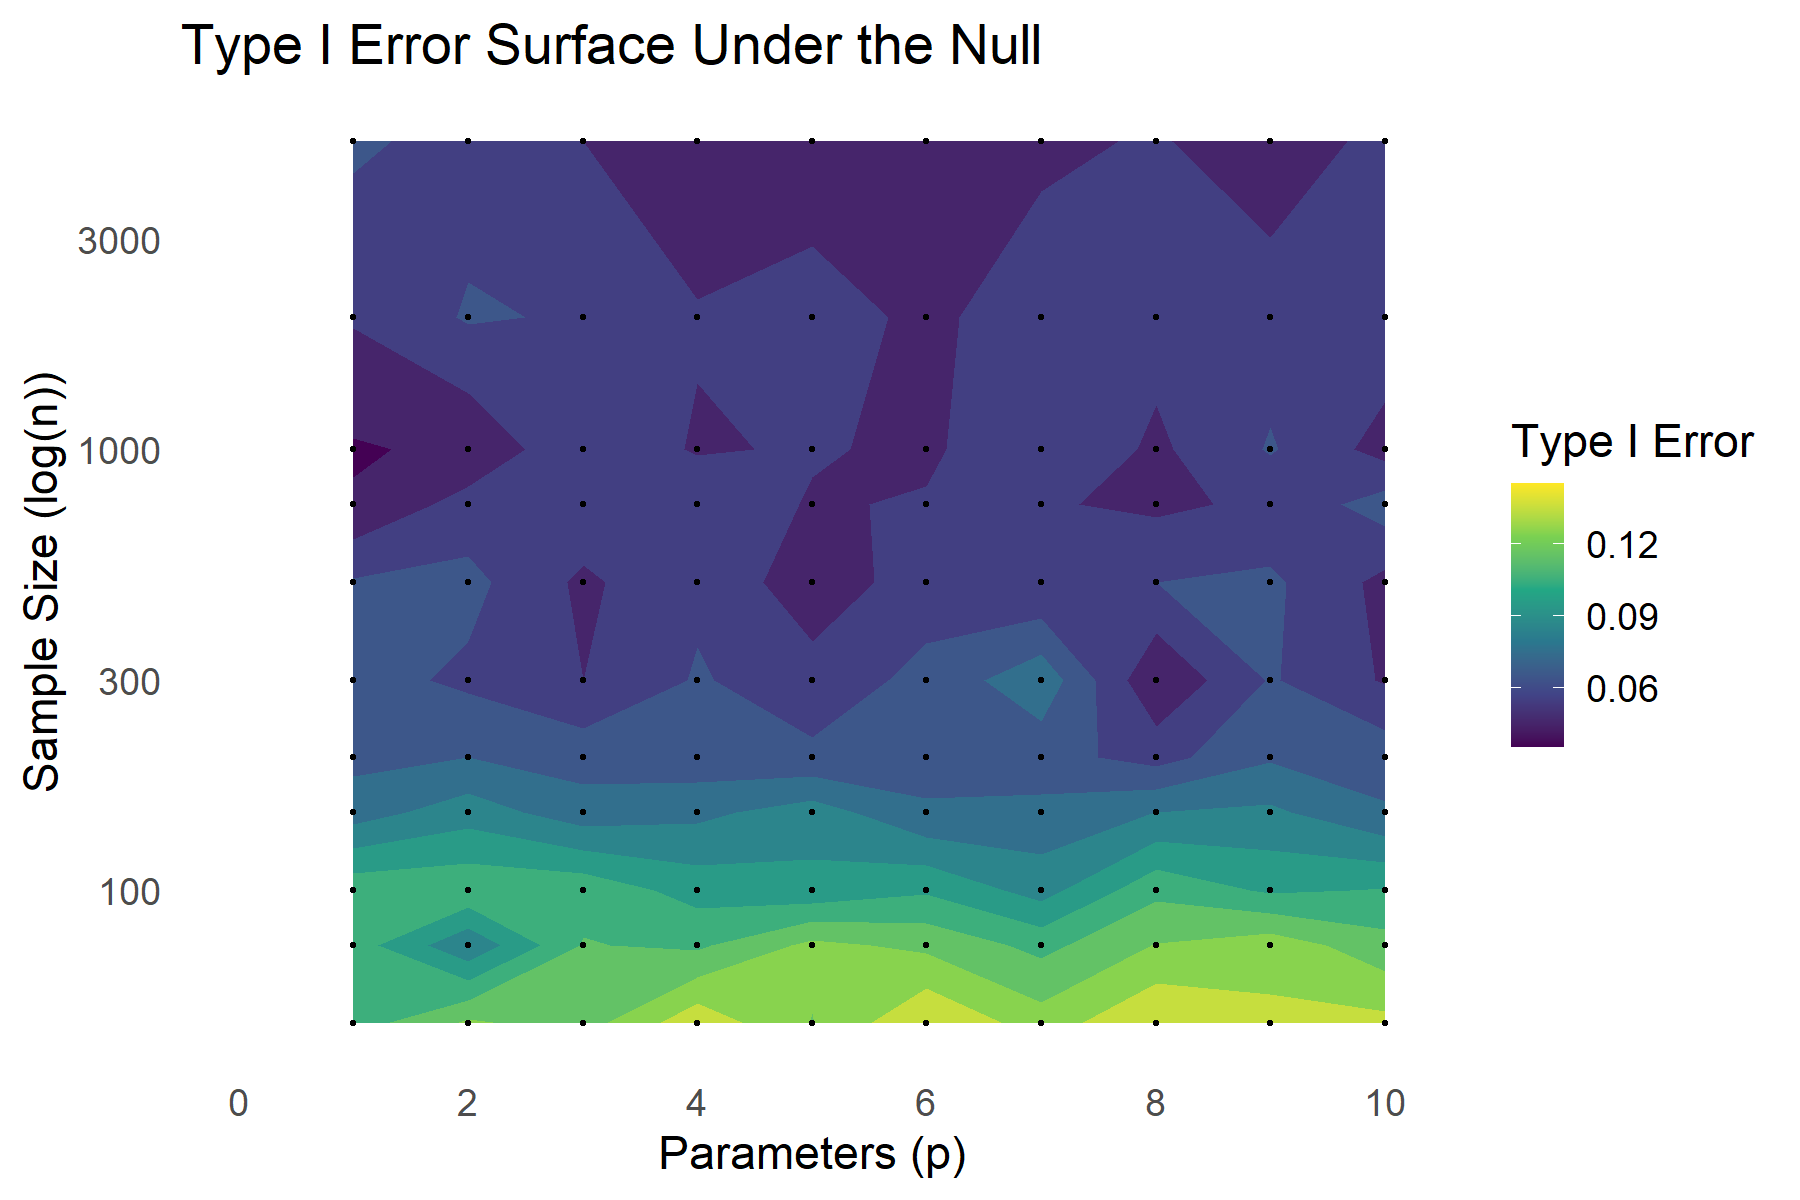
\includegraphics[width=0.92\linewidth]{Heatmap_MC} 

}

\caption{Empirical Type I error surface for the likelihood ratio test of a treatment-by-risk interaction across simulated sample sizes and numbers of prognostic covariates.}\label{fig:mc-type1-surface}
\end{figure}

Each point on the type I error surface represents the 1000 observations
of empirical type I error rate at that particular combination of
parameter and sample size values. The surface around each of these
points was interpolated using geom\_contour\_filled argument in
\texttt{ggplot2}. This linearly interpolates across the adjacent
observations to give approximate levels of type I error rates across the
entire surface. Type I error rates are notably higher in the lower
portion of the graph, representing sample size values below n = 300.
Within this region the empirical type one error rate lies in the
{[}0.09-0.12{]} range, and begins to stabilize towards 0.05 once sample
sizes are sufficiently large. A possible extension of this simulation
would be to examine whether a random forest approach to baseline risk
prediction yields even higher Type I error rates, as might be expected
from a more flexible modelling strategy. This simulation evidence aligns
with a recommended research area of the PATH statement, which stresses
the importance of identifying general principles, or heuristics to judge
the adequacy of sample sizes (David M. Kent et al. 2020).

\section{Discussion}\label{discussion}

The PATH statement, published in 2019, aimed to provide a framework for
and promotion of the implementation of predictive approaches to assess
the evidence of HTE within Randomised controlled-trials (David M. Kent
et al. 2020). Following this, the approach has been implemented to
various clinical datasets, largely in a retrospective manner, rather
than being packaged within the primary reporting of clinical trial
results. Our findings, from both empirical analyses of retrospective
datasets, as well simulation evidence may give an indication as to why
that is the case. Widespread implementation of PATH analyses may be
hindered by the necessity for an RCT to have an overall treatment
effect, RCT sample size limitations, relative complexity of the approach
and the absence of any regulatory expectations for predictive HTE
analyses in trial reporting.

From our empirical analyses, only the GUSTO-I trial and in a lesser
capacity the IST-I trial showed any evidence of heterogeneity of
treatment effect on the absolute scale. In contrast, the VITAL and DIG
trials showed little evidence of variation in absolute treatment effect
across baseline risk strata. This finding aligns with recommendations
from the PATH statement to apply risk-modeling approaches in the
presence of an overall treatment effect, and interpreted more cautiously
when there is not. The GUSTO-I trial reported a clear overall mortality
benefit of accelerated tPA compared with streptokinase (OR 0.85), while
the IST-I trial demonstrated a modest reduction in death or recurrent
stroke with aspirin (OR 0.95). By comparison, neither the DIG trial (RR
0.99 for all-cause mortality) nor the VITAL trial (HR 0.96 and 0.92 for
vitamin D and omega-3 supplementation, respectively) demonstrated a
clear overall treatment effect. In such settings, any genuine HTE in the
target population would need to take the form of a qualitative
interaction, where treatment is beneficial for some patients but harmful
for others, and such interactions are generally considered relatively
uncommon. The presence of heterogenous effects in the GUSTO-I and IST-I
trials supports the notion that meaning treatment effect heterogeneity
across risk-based subgroups is only likely to be found in trials
reporting an overall effect of an intervention on clinical outcomes.
Consequently, for trials that do not report any treatment effect, the
applicability of the PATH approach is lessened, which may contribute to
its relatively limited uptake since publication.

Another factor that may hinder the uptake of predictive approaches for
assessing treatment-effect heterogeneity is the requirement for
sufficiently large sample sizes. This limitation was highlighted in the
original PATH statement, with heuristics for identifying the adequacy of
sample sizes as a high-priority research need (David M. Kent et al.
2020). Our simulation evidence indicates that the likelihood of
detecting an interaction between baseline risk and treatment effect is
highly dependent on sample size. In particular, elevated empirical type
I error rates were detected in smaller datasets. This finding is also
consistent with the existing PATH literature, with the majority of
re-analyses of clinical trials using the PATH approach being employed
large clinical trial datasets (David M. Kent et al. 2016; Selby et al.
2025). Notably, many of these trials would fall outside the region of
elevated Type I error observed in our simulation surface. This apparent
requirement for large sample sizes may present a practical barrier to
the adoption of PATH analyses, particularly given the increasing
emphasis in clinical trial methodology on efficient study designs that
aim to answer research questions using the smallest sample size
compatible with adequate statistical power while minimizing research
costs. The necessity for an overall treatment effect to be present
alongside large, adequately powered sample sizes, narrows the
applicability of the PATH approach across contemporary clinical trials.

The lack of formal regulatory guidance on the incorporation of
predictive analyses for heterogeneity in the reporting of randomised
clinical trial results may also have contributed to the limited uptake
of the PATH framework. Historically, methodological advances in clinical
trial statistics often remain confined to the statistical literature
before becoming embedded within regulatory and reporting frameworks. The
estimand framework provides a recent example of this process.
Originating from efforts to improve the handling of missing data and
more precisely define treatment effects in clinical trials (Little et
al. 2012), the framework was subsequently formalised through the ICH
E9(R1) addendum in 2019. Despite this regulatory endorsement, uptake
remains incomplete, with a recent systematic review reporting that only
3\% of contemporary adaptive trial protocols explicitly specified a
primary estimand (Piazza et al. 2026). The uptake of the CONSORT
guidelines into RCT reporting provides a more successful case study.
First introduced in 1996 as a means of addressing incomplete and
inconsistent reporting of randomised controlled trials, the CONSORT
statement has undergone several revisions and updates, ultimately
becoming one of the most widely endorsed reporting frameworks in
clinical research (Hopewell et al. 2025). Evidence suggests that journal
endorsement of CONSORT is associated with improvements in the
completeness and transparency of trial reporting (Hopewell et al. 2025).
There remains an appetite for improving outcome reporting in a similar
manner to how we have challenged conventional trial reporting with both
the estimand and CONSORT frameworks. Whether PATH emerges as the
framework that addresses this gap will largely be determined by the
extent to which regulators and journals endorse and embed its principles
within clinical trial reporting requirements.

\subsection{Limitations and Future
work}\label{limitations-and-future-work}

Some critical constraints must be considered when interpreting findings
from this project. Data related limitations are the primary concern. In
the DIG trial we used the teaching dataset,in which most variables were
permuted over the set of patients within treatment groups to make sure
complete anonymisation was maintained. This permutation process means
that multidimensional relationships are not explicitly documented in the
original report and may not have been preserved. As a result the
validity of multivariate inferences derived from this specific teaching
dataset are compromised. Furthermore, while the National Lung Screening
Trial (NLST) (null 2011) was initially targeted to evaluate the PATH
framework in the oncology space, the inavailability of NLST data
necessiated a transition to the VITAL trial dataset for the final
empirical analysis.

Beyond these, this project is subject to the inherent lack of
statistical power for interaction test in conventional RCTs, which are
primarily designed to detect average treatment effects rather than
heterogeneity(Senn and Hahn 2026). There may be limited power to detect
genuine variation in large trials including GUSTO-I which leads to a
risk of false negatives(Type I errors)(Califf et al. 1997). In addition,
since patients in these parallel arm trials only receive one
intervention, individual treatment effects are technically unobservable,
as a result the models provide conditional average treatment effects for
reference classes rather than direct measures of a unique individual's
response (David M. Kent et al. 2020; David M. Kent, Steyerberg, and Van
Klaveren 2018).

Future work may move beyond primary outcome risk by integrating
treatment-related harms into predictive models, allowing benefit--harm
trade-off analyses across different risk strata (David M. Kent et al.
2020; David M. Kent, Steyerberg, and Van Klaveren 2018). To strengthen
the clinical credibility of these findings, the identified models should
undergo external validation and calibration in independent patient
cohorts to ensure applicability to real-world populations (Selby et al.
2025; David M. Kent et al. 2020). Methodologically, future research
should implement decision curve analysis to evaluate whether a strategy
of treating only those above a specific risk threshold is superior to
treating all patients (Selby et al. 2025; David M. Kent et al. 2020).
Finally, further investigation is required to determine whether
tree-based machine learning algorithms, including causal forests,
provide distinct predictive advantages over traditional regression-based
approaches for identifying patient-specific treatment benefit in these
clinical contexts (David M. Kent et al. 2020; David M. Kent, Steyerberg,
and Van Klaveren 2018).

\section{Conclusion}\label{conclusion}

Seven years after the initial publication of the PATH statement by Kent
and colleagues, there is strong evidence that the approach facilitates
more informative reporting of heterogeneity of treatment effects within
clinical trial populations (David M. Kent et al. 2020). Our analyses
provided further evaluation of the PATH framework and supported several
of its recommendations, particularly the use of large clinical trials
with favourable overall treatment effects. Through a simulation study,
we also examined the role of sample size, observing inflated empirical
type I error rates in smaller samples, consistent with concerns raised
in the original elaboration document. A natural next step is to further
define the characteristics of clinical trials that are most suitable for
the PATH approach, including how the magnitude of the overall treatment
effect influences the ability to detect HTE.

The PATH approach offers clear advantages over traditional, one variable
at a time methods for exploring HTE within trial populations. However,
application of the approach remains confined to post-facto analyses,
including those presented here, with a distinct lack of implementation
within newly published RCTs. Bridging the gap from statistical
methodology to real-world application, will require adoption from trial
investigators, endorsement from journals and potentially guidance from
regulatory bodies. Future work should therefore focus on not only
refining the statistical implementation of the approach, but also
identifying practical ways to integrate it into prospective trial
design.

\section{CRediT Author Statement}\label{credit-author-statement}

Tom Delany: Methodology, Software, Formal analysis, Investigation, Data
curation, Writing - Original Draft, Writing - Review \& Editing,
Visualization.

Misgana Ojamo: Methodology, Software, Formal analysis, Investigation,
Data curation, Writing - Original Draft, Writing - Review \& Editing,
Visualization.

Neil O'Leary: Conceptualization, Supervision, Writing - Review \&
Editing.

\section{Acknowledgements}\label{acknowledgements}

We would like to thank Dr.~Neil O'Leary for his support throughout the
year, both in advising us on this thesis and in helping with questions
that arose in relation to other coursework and career matters.

\section{References}\label{references}

\phantomsection\label{refs}
\begin{CSLReferences}{1}{0}
\bibitem[\citeproctext]{ref-InternationalRandomizedTrial1993}
{``An {International Randomized Trial Comparing Four Thrombolytic
Strategies} for {Acute Myocardial Infarction}.''} 1993. \emph{New
England Journal of Medicine} 329 (10): 673--82.
\url{https://doi.org/10.1056/NEJM199309023291001}.

\bibitem[\citeproctext]{ref-10.1093ux2fbiometux2fasaf029}
Bannick, Marlena S, Jun Shao, Jingyi Liu, Yu Du, Yanyao Yi, and Ting Ye.
2025. {``A General Form of Covariate Adjustment in Clinical Trials Under
Covariate-Adaptive Randomization.''} \emph{Biometrika} 112 (3): asaf029.
\url{https://doi.org/10.1093/biomet/asaf029}.

\bibitem[\citeproctext]{ref-bellavia_heterogeneity_2024}
Bellavia, Andrea, and Sabina A. Murphy. 2024. {``Heterogeneity of
{Treatment} {Effects} in {Clinical} {Trials}: {Overview} of
{Multivariable} {Approaches} and {Practical} {Recommendations}.''}
\emph{Circulation} 150 (13): 978--80.
\url{https://doi.org/10.1161/CIRCULATIONAHA.124.069857}.

\bibitem[\citeproctext]{ref-caldeiraFishIntakeRisk2023}
Caldeira, Daniel, Beatriz Nogueira-Garcia, Ana Abreu, and Fausto J.
Pinto. 2023. {``Fish Intake and Risk of Cardiovascular Events: An
Analysis of the {VITAL} Cohort.''} \emph{European Journal of Clinical
Nutrition} 77 (3): 400--404.
\url{https://doi.org/10.1038/s41430-022-01244-w}.

\bibitem[\citeproctext]{ref-califf_selection_1997}
Califf, Robert M., Lynn H. Woodlief, Frank E. Harrell, Kerry L. Lee,
Harvey D. White, Alan Guerci, Gabriel I. Barbash, et al. 1997.
{``Selection of Thrombolytic Therapy for Individual Patients:
{Development} of a Clinical Model.''} \emph{American Heart Journal} 133
(6): 630--39. \url{https://doi.org/10.1016/S0002-8703(97)70164-9}.

\bibitem[\citeproctext]{ref-cuzickForestPlotsInterpretation2005}
Cuzick, Jack. 2005. {``Forest Plots and the Interpretation of
Subgroups.''} \emph{The Lancet} 365 (9467): 1308.
\url{https://doi.org/10.1016/S0140-6736(05)61026-4}.

\bibitem[\citeproctext]{ref-zotero-item-39}
Daniels, Gilbert S. 1952. {``The "{Average Man}"?''} WADC TN 53-7.
Wright-Patterson Air Force Base, Ohio: {Wright Air Development Center,
Air Research and Development Command, United States Air Force}.

\bibitem[\citeproctext]{ref-dessaiTestingInterpretingAssumptions2019}
Dessai, Sampada, and Vijay Patil. 2019. {``Testing and Interpreting
Assumptions of {COX} Regression Analysis.''} \emph{Cancer Research,
Statistics, and Treatment} 2 (1).

\bibitem[\citeproctext]{ref-gabler_dealing_2009}
Gabler, Nicole B, Naihua Duan, Diana Liao, Joann G Elmore, Theodore G
Ganiats, and Richard L Kravitz. 2009. {``Dealing with Heterogeneity of
Treatment Effects: Is the Literature up to the Challenge?''}
\emph{Trials} 10 (1): 43. \url{https://doi.org/10.1186/1745-6215-10-43}.

\bibitem[\citeproctext]{ref-greenfield_heterogeneity_2007}
Greenfield, Sheldon, Richard Kravitz, Naihua Duan, and Sherrie H.
Kaplan. 2007. {``Heterogeneity of {Treatment} {Effects}: {Implications}
for {Guidelines}, {Payment}, and {Quality} {Assessment}.''} \emph{The
American Journal of Medicine} 120 (4): S3--9.
\url{https://doi.org/10.1016/j.amjmed.2007.02.002}.

\bibitem[\citeproctext]{ref-10.1001ux2fjama.2025.4347}
Hopewell, Sally, An-Wen Chan, Gary S. Collins, Asbjørn Hróbjartsson,
David Moher, Kenneth F. Schulz, Ruth Tunn, et al. 2025. {``{CONSORT}
2025 Statement: {Updated} Guideline for Reporting Randomized Trials.''}
\emph{JAMA : The Journal of the American Medical Association} 333 (22):
1998--2005. \url{https://doi.org/10.1001/jama.2025.4347}.

\bibitem[\citeproctext]{ref-hwangboStackingEnsembleLearning2022}
Hwangbo, Lee, Yoon Jung Kang, Hoon Kwon, Jae Il Lee, Han-Jin Cho,
Jun-Kyeung Ko, Sang Min Sung, and Tae Hong Lee. 2022. {``Stacking
Ensemble Learning Model to Predict 6-Month Mortality in Ischemic Stroke
Patients.''} \emph{Scientific Reports} 12 (1): 17389.
\url{https://doi.org/10.1038/s41598-022-22323-9}.

\bibitem[\citeproctext]{ref-janssenSimpleMethodAdjust2009}
Janssen, Kristel J. M., Yvonne Vergouwe, Cor J. Kalkman, Diederick E.
Grobbee, and Karel G. M. Moons. 2009. {``A Simple Method to Adjust
Clinical Prediction Models to Local Circumstances.''} \emph{Canadian
Journal of Anesthesia/Journal Canadien d'anesthésie} 56 (3): 194--201.
\url{https://doi.org/10.1007/s12630-009-9041-x}.

\bibitem[\citeproctext]{ref-JONES20041025}
Jones, R. Christopher, Gary S. Francis, and Michael S. Lauer. 2004.
{``Predictors of Mortality in Patients with Heart Failure and Preserved
Systolic Function in the {Digitalis Investigation Group} Trial.''}
\emph{Journal of the American College of Cardiology} 44 (5): 1025--29.
\url{https://doi.org/10.1016/j.jacc.2004.05.077}.

\bibitem[\citeproctext]{ref-10.1093ux2fijeux2fdyw118}
Kent, David M, Jason Nelson, Issa J Dahabreh, Peter M Rothwell, Douglas
G Altman, and Rodney A Hayward. 2016. {``Risk and Treatment Effect
Heterogeneity: Re-Analysis of Individual Participant Data from 32 Large
Clinical Trials.''} \emph{International Journal of Epidemiology} 45 (6):
2075--88. \url{https://doi.org/10.1093/ije/dyw118}.

\bibitem[\citeproctext]{ref-kent_assessing_2010}
Kent, David M, Peter M Rothwell, John Pa Ioannidis, Doug G Altman, and
Rodney A Hayward. 2010. {``Assessing and Reporting Heterogeneity in
Treatment Effects in Clinical Trials: A Proposal.''} \emph{Trials} 11
(1): 85. \url{https://doi.org/10.1186/1745-6215-11-85}.

\bibitem[\citeproctext]{ref-kent_personalized_2018}
Kent, David M, Ewout Steyerberg, and David Van Klaveren. 2018.
{``Personalized Evidence Based Medicine: Predictive Approaches to
Heterogeneous Treatment Effects.''} \emph{BMJ}, December, k4245.
\url{https://doi.org/10.1136/bmj.k4245}.

\bibitem[\citeproctext]{ref-kent_predictive_2020}
Kent, David M., David Van Klaveren, Jessica K. Paulus, Ralph D'Agostino,
Steve Goodman, Rodney Hayward, John P. A. Ioannidis, et al. 2020. {``The
{Predictive} {Approaches} to {Treatment} Effect {Heterogeneity} ({PATH})
{Statement}: {Explanation} and {Elaboration}.''} \emph{Annals of
Internal Medicine} 172 (1): W1--25.
\url{https://doi.org/10.7326/M18-3668}.

\bibitem[\citeproctext]{ref-doi:10.1056ux2fNEJMsr1203730}
Little, Roderick J., Ralph D'Agostino, Michael L. Cohen, Kay Dickersin,
Scott S. Emerson, John T. Farrar, Constantine Frangakis, et al. 2012.
{``The Prevention and Treatment of Missing Data in Clinical Trials.''}
\emph{New England Journal of Medicine} 367 (14): 1355--60.
\url{https://doi.org/10.1056/NEJMsr1203730}.

\bibitem[\citeproctext]{ref-Matsuki02012016}
Matsuki, Kazunaga, Victor Kuperman, and Julie A. Van Dyke. 2016. {``The
{Random Forests} Statistical Technique: {An} Examination of Its Value
for the Study of Reading.''} \emph{Scientific Studies of Reading} 20
(1): 20--33. \url{https://doi.org/10.1080/10888438.2015.1107073}.

\bibitem[\citeproctext]{ref-https:ux2fux2fdoi.orgux2f10.1002ux2fsim.8086}
Morris, Tim P., Ian R. White, and Michael J. Crowther. 2019. {``Using
Simulation Studies to Evaluate Statistical Methods.''} \emph{Statistics
in Medicine} 38 (11): 2074--2102.
\url{https://doi.org/10.1002/sim.8086}.

\bibitem[\citeproctext]{ref-doi:10.1056ux2fNEJMoa1102873}
null, null. 2011. {``Reduced Lung-Cancer Mortality with Low-Dose
Computed Tomographic Screening.''} \emph{New England Journal of
Medicine} 365 (5): 395--409.
\url{https://doi.org/10.1056/NEJMoa1102873}.

\bibitem[\citeproctext]{ref-piazzaInvestigatingEstimandConsiderations2026}
Piazza, Fran, Hannah Wallace, Rachel Phillips, Suzie Cro, and Zohra
Zenasni. 2026. {``Investigating Estimand Considerations in Adaptive
Trials: A Systematic Review.''} \emph{Trials} 27 (1): 197.
\url{https://doi.org/10.1186/s13063-026-09490-0}.

\bibitem[\citeproctext]{ref-rose_end_2016}
Rose, T. 2016. \emph{The {End} of {Average}: {How} {We} {Succeed} in a
{World} {That} {Values} {Sameness}}. HarperCollins.
\url{https://books.google.ie/books?id=0gxXrgEACAAJ}.

\bibitem[\citeproctext]{ref-selby_predictive_2025}
Selby, Joe V., Carolien C. H. M. Maas, Bruce H. Fireman, and David M.
Kent. 2025. {``Predictive {Modeling} of {Heterogeneous} {Treatment}
{Effects} in {RCTs}: {A} {Scoping} {Review}.''} \emph{JAMA Network Open}
8 (7): e2522390.
\url{https://doi.org/10.1001/jamanetworkopen.2025.22390}.

\bibitem[\citeproctext]{ref-senn_heterogeneous_2026}
Senn, Stephen, and Richard Hahn. 2026. {``Do {Heterogeneous} {Treatment}
{Effects} {Exist}?''} \url{https://www.youtube.com/watch?v=V801RQTBpp4}.

\bibitem[\citeproctext]{ref-STEYERBERG2000745}
Steyerberg, Ewout W., Patrick M. M. Bossuyt, and Kerry L. Lee. 2000.
{``Clinical Trials in Acute Myocardial Infarction: {Should} We Adjust
for Baseline Characteristics?''} \emph{American Heart Journal} 139 (5):
745--51. \url{https://doi.org/10.1016/S0002-8703(00)90001-2}.

\bibitem[\citeproctext]{ref-sun_is_2010}
Sun, X., M. Briel, S. D. Walter, and G. H. Guyatt. 2010. {``Is a
Subgroup Effect Believable? {Updating} Criteria to Evaluate the
Credibility of Subgroup Analyses.''} \emph{BMJ} 340 (mar30 3): c117--17.
\url{https://doi.org/10.1136/bmj.c117}.

\bibitem[\citeproctext]{ref-thompsonCovariateAdjustmentHad2015}
Thompson, Douglas D., Hester F. Lingsma, William N. Whiteley, Gordon D.
Murray, and Ewout W. Steyerberg. 2015. {``Covariate Adjustment Had
Similar Benefits in Small and Large Randomized Controlled Trials.''}
\emph{Journal of Clinical Epidemiology} 68 (9): 1068--75.
\url{https://doi.org/10.1016/j.jclinepi.2014.11.001}.

\bibitem[\citeproctext]{ref-varadhan_estimation_2013}
Varadhan, R, and JD Seeger. 2013. {``Estimation and {Reporting} of
{Heterogeneity} of {Treatment} {Effects}.''} In \emph{Developing a
{Protocol} for {Observational} {Comparative} {Effectiveness} {Research}:
{A} {User}'s {Guide}.} Rockville (MD): Agency for Healthcare Research;
Quality (US).

\bibitem[\citeproctext]{ref-JSSv036i03}
Viechtbauer, Wolfgang. 2010. {``Conducting Meta-Analyses in {R} with the
Metafor Package.''} \emph{Journal of Statistical Software} 36 (3):
1--48. \url{https://doi.org/10.18637/jss.v036.i03}.

\bibitem[\citeproctext]{ref-wang_statistics_2007}
Wang, Rui, Stephen W. Lagakos, James H. Ware, David J. Hunter, and
Jeffrey M. Drazen. 2007. {``Statistics in {Medicine} --- {Reporting} of
{Subgroup} {Analyses} in {Clinical} {Trials}.''} \emph{New England
Journal of Medicine} 357 (21): 2189--94.
\url{https://doi.org/10.1056/NEJMsr077003}.

\bibitem[\citeproctext]{ref-willke_concepts_2012}
Willke, Richard J, Zhiyuan Zheng, Prasun Subedi, Rikard Althin, and C
Daniel Mullins. 2012. {``From Concepts, Theory, and Evidence of
Heterogeneity of Treatment Effects to Methodological Approaches: A
Primer.''} \emph{BMC Medical Research Methodology} 12 (1): 185.
\url{https://doi.org/10.1186/1471-2288-12-185}.

\bibitem[\citeproctext]{ref-JSSv077i01}
Wright, Marvin N., and Andreas Ziegler. 2017. {``Ranger: A Fast
Implementation of Random Forests for High Dimensional Data in {C}++ and
{R}.''} \emph{Journal of Statistical Software} 77 (1): 1--17.
\url{https://doi.org/10.18637/jss.v077.i01}.

\end{CSLReferences}

\bibliographystyle{unsrt}
\bibliography{PATH\_intro\_references.bibPATH - Thesis/MSc -Thesis.bib}


\end{document}
